\documentclass[a4paper,papersize,dvipdfmx]{mtabst}
\usepackage{graphicx}
\usepackage{amsmath}
\usepackage{times}
%\usepackage{jumoline}
\usepackage{type1cm}
\usepackage{bm}
\usepackage{url}
\usepackage{subcaption}
%\usepackage{secdot}
%\usepackage{mystyle}
% \usepackage{subfig} % subfigure.sty は古いので避けた方がよい.
% \usepackage[tight]{subfigure}

\pagestyle{fancy}

\chead{} % ヘッダは印刷業者がつけるので記入しない
%\chead{\sffamily \gtfamily 横浜国立大学大学院 機械システム工学コース 学位論文概要集,Vol.?,20??} % その年の指定に合わせて変更

% \newcommand{\secref}[1]{\ref{#1}章}
\newcommand{\ssecref}[1]{\ref{#1}節}
\newcommand{\figref}[1]{Fig.~\ref{#1}}
% \newcommand{\tabref}[1]{表~\ref{#1}}
\renewcommand{\eqref}[1]{式~(\ref{#1})}

\setlength\intextsep{0pt}
\setlength\textfloatsep{0pt}

\begin{document}
\date{}

\title{平面内センサレスin-handケージングマニピュレーションの計画}

\etitle{Planning of Planar Sensorless In-hand Caging Manipulation}

\author{
\begin{tabular}{p{.45\linewidth}p{.45\linewidth}}
\centering \gtfamily{21NA140 中西 佑太} & \centering (\gtfamily{主査 前田 雄介 教授})
\end{tabular}
}

\eauthor{
\begin{tabular}{p{.45\linewidth}p{.45\linewidth}}
\centering 21NA140 Yuta NAKANISHI & \centering (Supervisor Prof. Yusuke MAEDA)
\end{tabular}
}

\keywords{Manipulation, Robot hand, Motion planning}

\begin{abstract}
In this work I developed a planner for planar sensorless in-hand caging manipulation.
In-hand caging manipulation is a method in which an object is caged by a hand throughout manipulation and located around a goal as a result of the deformation of the cage without sensing the object configuration.
This method can be applied to part feeders to manipulate objects from random to targeted poses. 
In this paper, the following three points were proposed, a new robot hand configuration named ``opposite-type hand'', new motion planning algorithms and a post motion planner for positioning.
The first aims to make the manipulation more robust. 
The second improves calculation time and pose accuracy and allows users to select the appropriate algorithm for their needs.
The third improves pose accuracy furthermore by closing the robot hand until the object reaches desired pose after planning.
Experimental results demonstrated the effectiveness of the proposed points. 
\end{abstract}

\maketitle
%\thispagestyle{fancy}

\section{序論}
In-handマニピュレーションは手の中で物体の位置や向きを変化させる動作である.これをロボットハンドで再現した研究の多くはカメラや力センサなどでセンシングし,実現されている.一方,物体の拘束手法の一つにケージング\cite{rimon1999}というものがある.これは,対象物が逃げられないように幾何学的に囲い込む拘束手法であり,ハンドの位置制御のみで物体を拘束でき,力センサを必要としないという特徴がある.\par
本研究グループではこれらを組み合わせた「センサレスIn-handケージングマニピュレーション」を提案している.ケージングを維持しつつロボットハンドによる囲いの形状を適切に変化させていくことで,力センシングや力制御なしでマニピュレーションを実現できる.先行研究\cite{komiyama2021}では,1. 対象物がハンドに詰まることでハンドを正常に動かせなくなる「ジャミング」が発生する,2. 動作計画に長い計算時間がかかる,3. 位置決め精度が十分でない,といった課題が存在した.そこで本研究では,これらの課題を解決することを目的とする.


\section{システムの全体像}
\subsection{汎用パーツフィーダ \cite{kamikukita2022}}
本手法は,位置・姿勢にばらつきのある対象物を特定の位置・姿勢に整列できるという機能を活かして汎用パーツフィーダへ応用することを考えている.そこで,ベルトコンベアと1対のロボットハンドを用いて\figref{fig::partfeeder}のようなシステムを構築した.ロボットハンドは,3つのリンクと3つの関節からなる3自由度ハンドで,これを並列させることで1対のロボットハンドを構成している.リンクは3Dプリンタで作成し,関節にはサーボモータを用いている.以降,このハンド構成を並列型ハンドと呼ぶこととする.

\subsection{対向型ハンド}
並列型ハンド\cite{komiyama2021},\cite{kamikukita2022}には次の2つの問題があった.一つは\figref{fig::jam}(b)(c)のように根元付近に対象物が詰まり,ハンドが動けなくなる「ジャミング」が発生していた点,もう一つは構造上,ハンド根元付近の物体をマニピュレーションできないという点である.これらは並列型ハンドにおいて一般的に起こりうるが,センサを用いて指先付近で操ればあまり問題にならない.しかし,本研究のようなセンサレスin-handケージングマニピュレーションでは回避が困難である.\par
これらの問題の解消に向け,\figref{fig::oppositehand}のようなハンド構成,対向型ハンドを提案する.前者の問題に関しては,ジャミングの原因となっていたパーム部付近のハンド自由度の低い領域が対向型ハンドには存在しないことから解決が見込める.後者の問題に関しても,一方のハンドの根元側に物体があったとしても,他方のハンドで掬い取るような動作で対応可能である.

\begin{figure}[t]
	\centering
	\begin{minipage}{0.7\linewidth}
	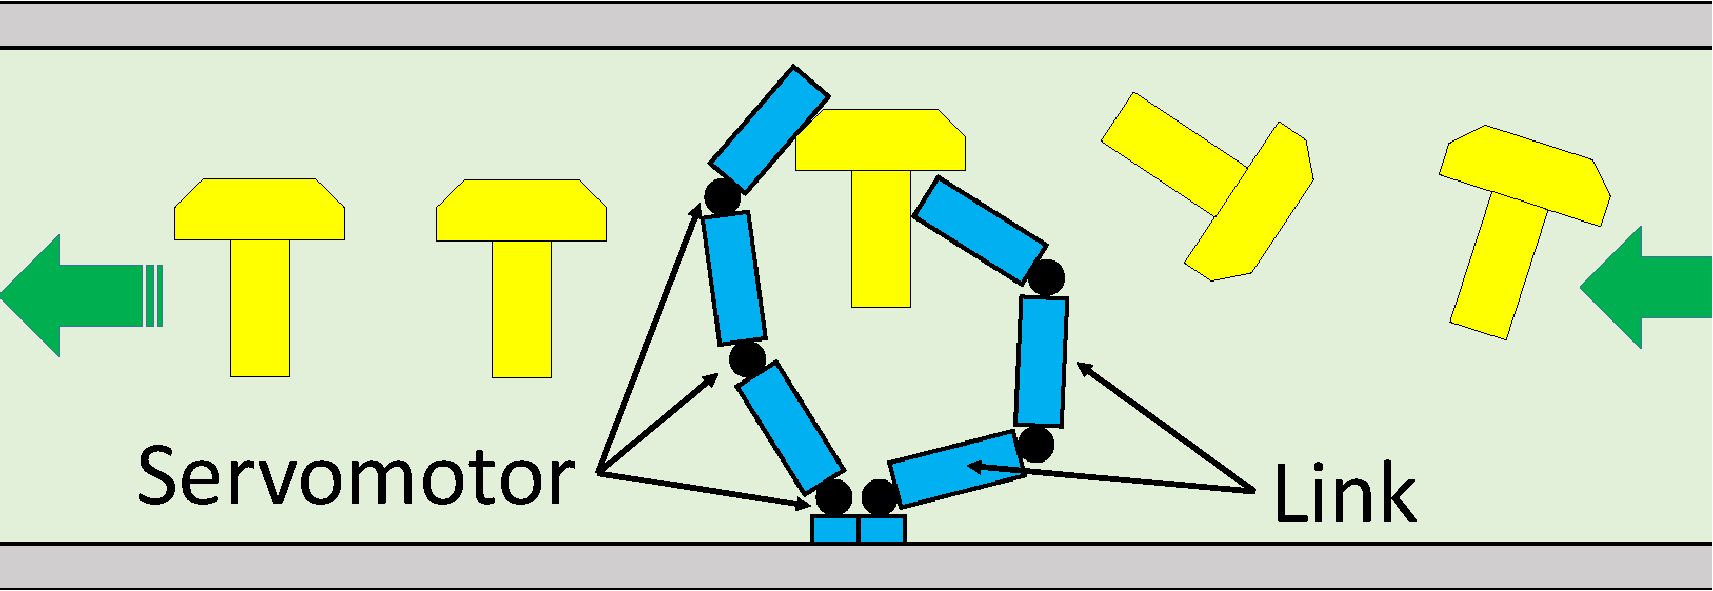
\includegraphics[width=0.9\linewidth]{fig/abstract/part_feeder.pdf}
	\caption{applying to part feeders}
	\label{fig::partfeeder}
	\end{minipage}\hfill
	\begin{minipage}{0.29\linewidth}
	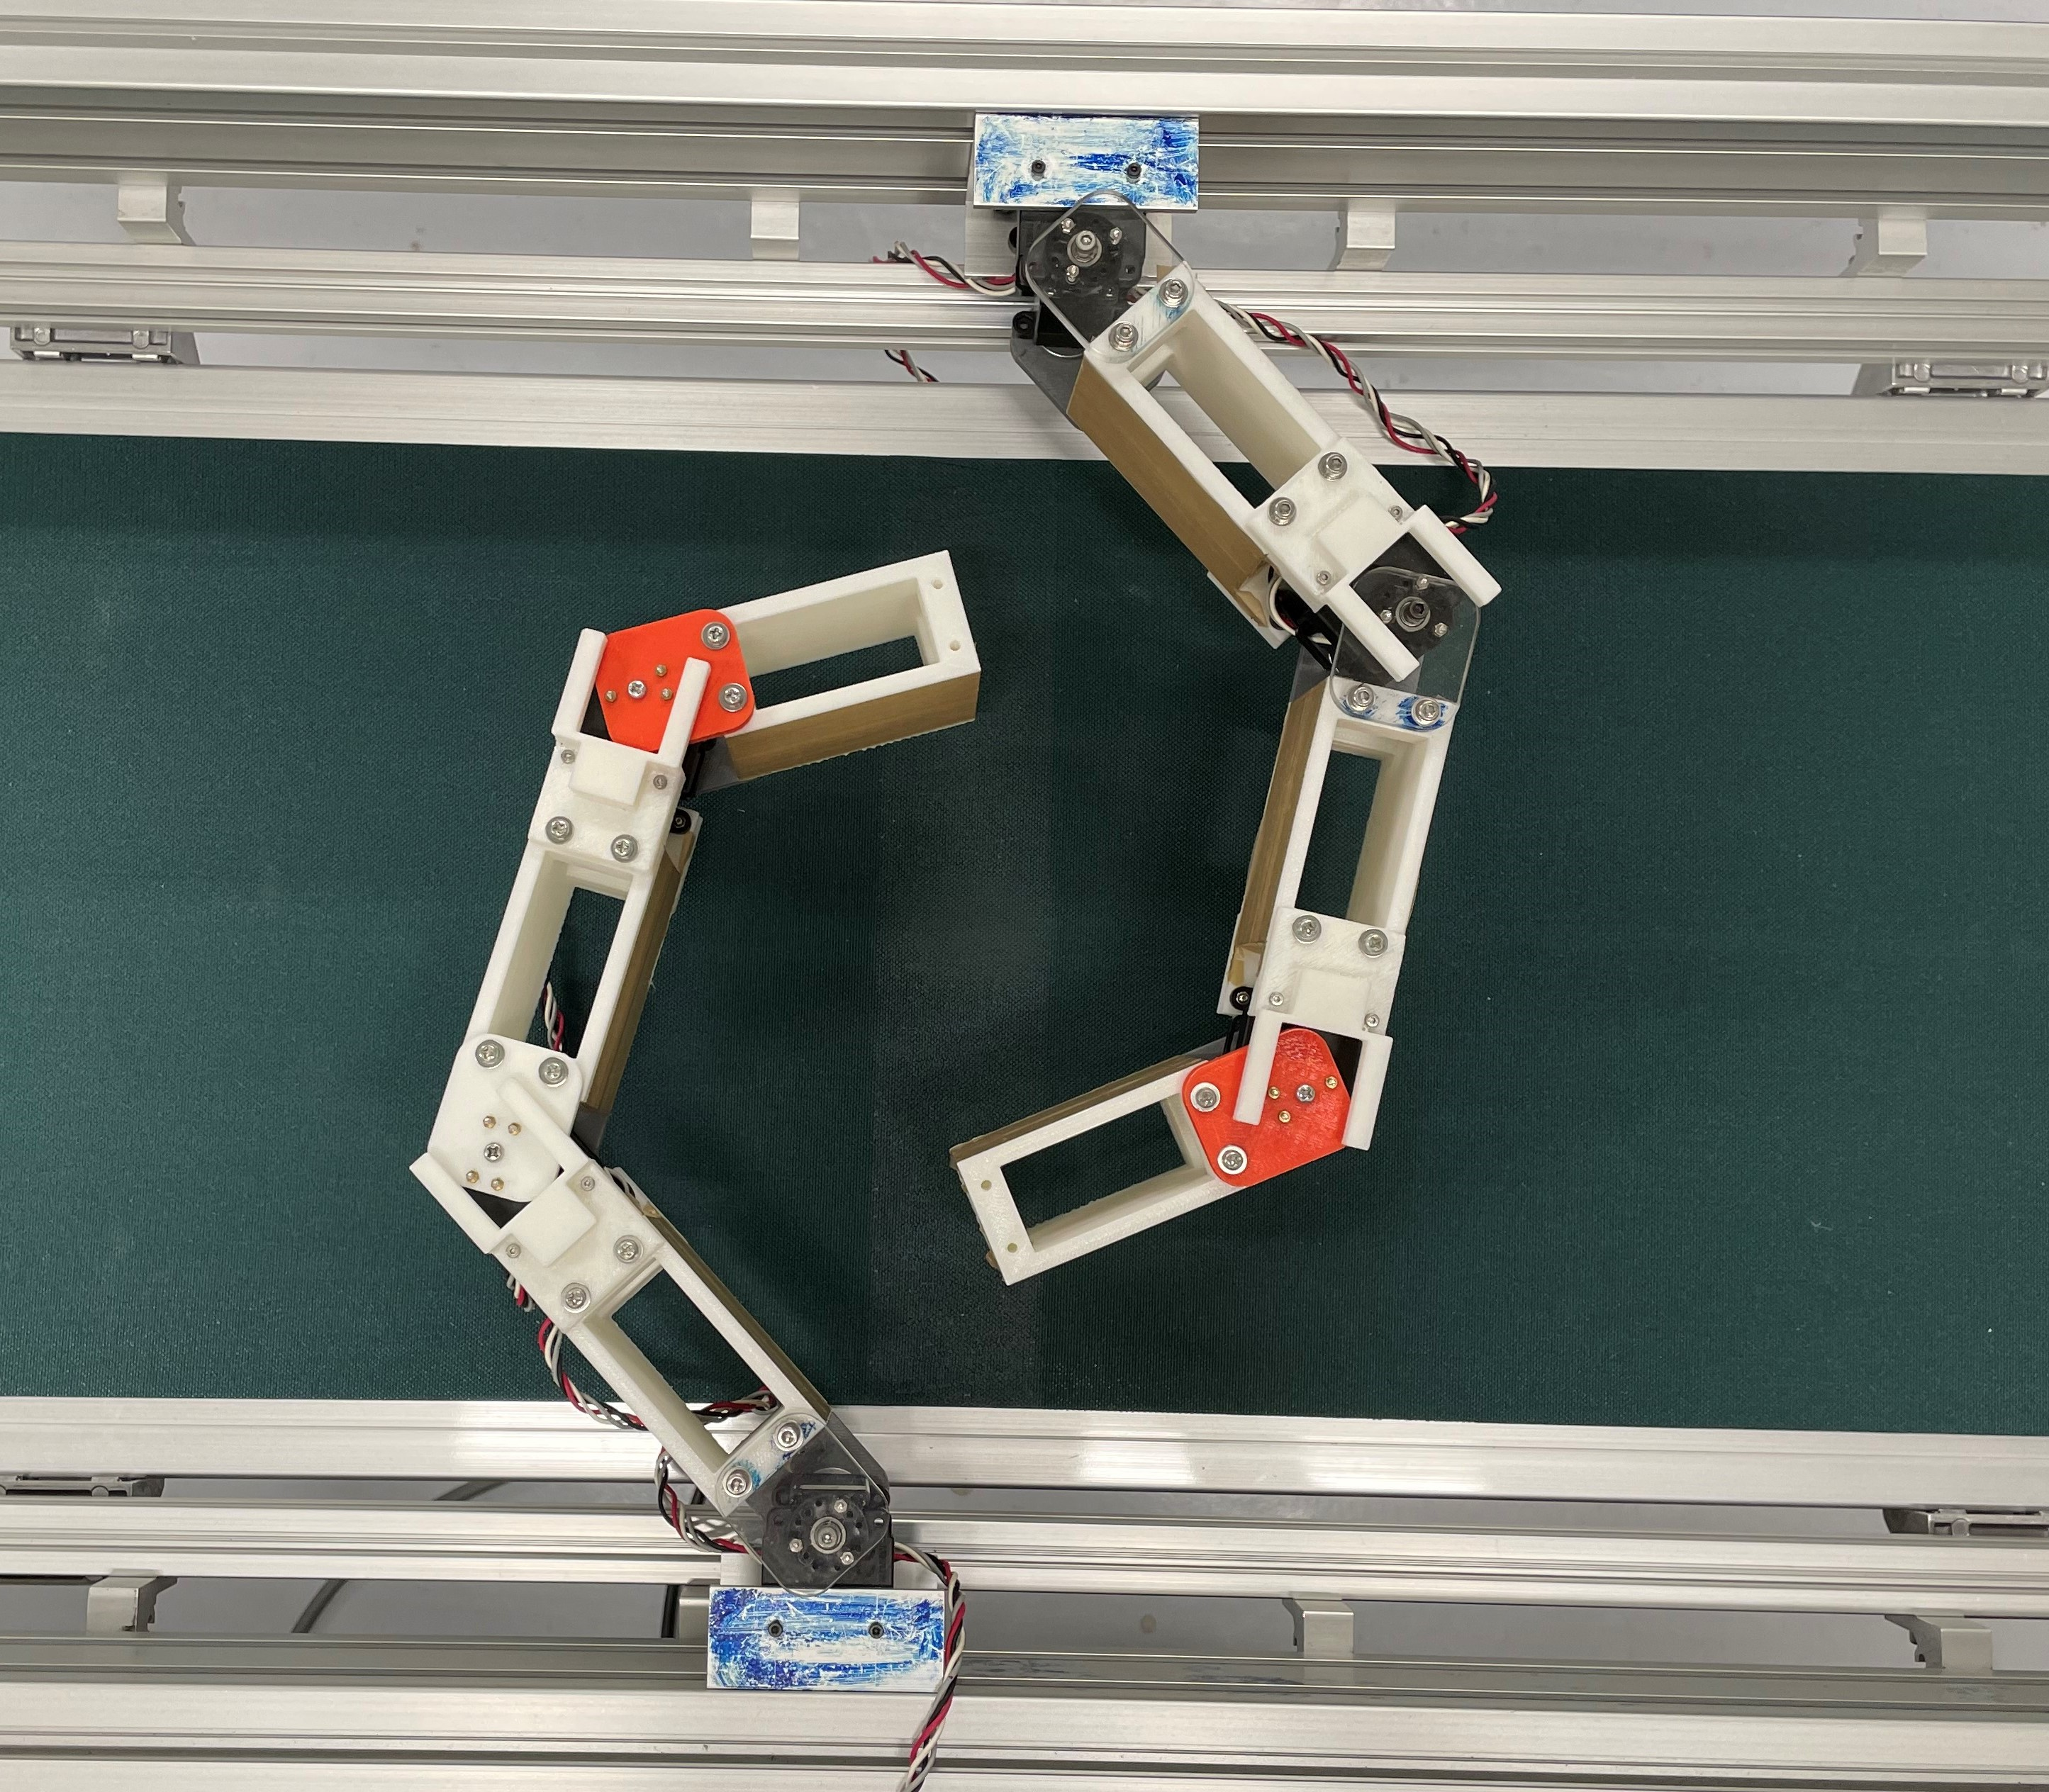
\includegraphics[width=0.95\linewidth]{fig/abstract/opposite2.jpg}
	\caption{Opposite-type hand}
	\label{fig::oppositehand}
	\end{minipage}
	
	\begin{minipage}{0.33\linewidth}
	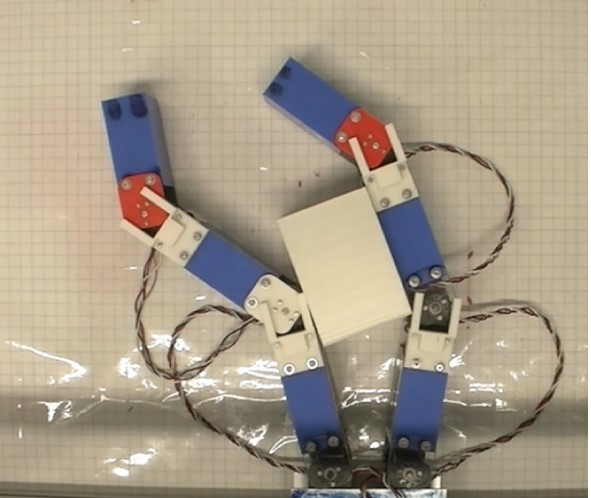
\includegraphics[width=0.85\linewidth]{fig/abstract/parallel1.jpg}
	\subcaption{before jam}
	\end{minipage}\hfill
	\begin{minipage}{0.33\linewidth}
	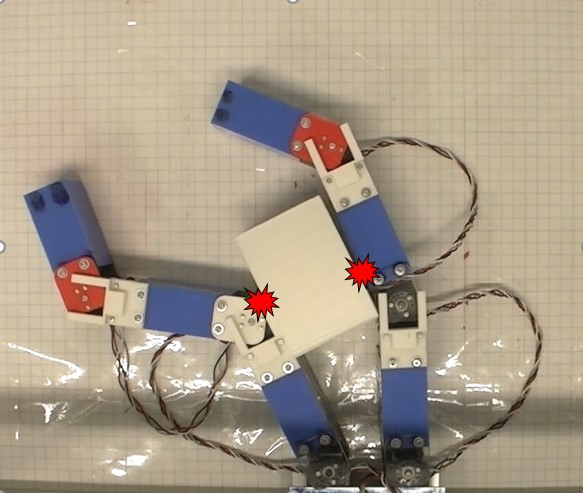
\includegraphics[width=0.85\linewidth]{fig/abstract/parallel2.jpg}
	\subcaption{just jammed}
	\end{minipage}\hfill
	\begin{minipage}{0.33\linewidth}
	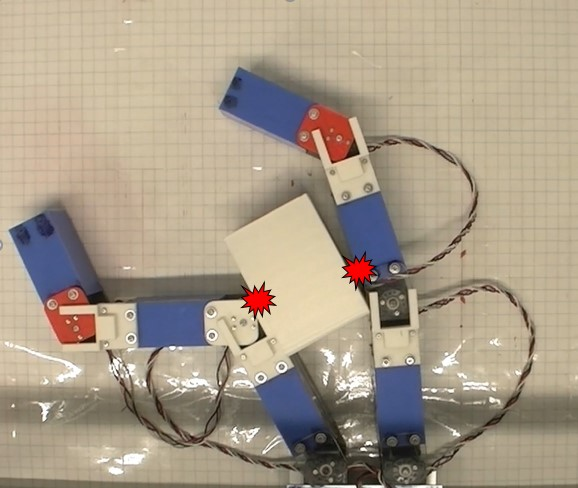
\includegraphics[width=0.85\linewidth]{fig/abstract/parallel3.jpg}
	\subcaption{still jammed}
	\end{minipage}
	\caption{Manipulation by parallel-type hand (Jamming occuring)}\label{fig::jam}
\end{figure}


\section{動作計画アルゴリズム}
本動作計画プログラムは,対象物の形状情報,目標位置・姿勢などを入力として与えると,出力としてハンドの動かし方が得られるというものになっている.
本手法ではセンサを用いないため,動作計画の際,対象物の正確な位置・姿勢情報を使うことはできない.しかし,あるハンド姿勢に対して,ハンド内部で対象物が取れる位置・姿勢群は計算できる.これを対象物の存在領域$\mathcal{C}_{\mathrm {free\_obj}}$と呼ぶ.適切なハンドの動かし方を探索し,$\mathcal{C}_{\mathrm {free\_obj}}$を徐々に減らしていき,最終的に$\mathcal{C}_{\mathrm {free\_obj}}$が目標位置・姿勢とその周辺のみを取るような状態を目指す.これにより,センサレスに対象物をゴールまでマニピュレーションすることができる.\par 

\subsection{順探索アルゴリズム}	\label{rrt}
ハンドの動かし方は,RRT (Rapidly-exploring Random Tree)を用いて探索する.探索空間は,ハンドの関節角度6個からなる6自由度空間となっている.探索開始点には任意のマニピュレーション初期姿勢を与える.その過程の各ノードにおいて,ケージング維持のために満たすべき条件を確認し,満足しているものだけを妥当なノードとして追加していく.探索終了条件は$\mathcal{C}_{\mathrm {free\_obj}}$が目標位置・姿勢$P_G(x_{\mathrm{any}}, y_G, \phi_G )$付近で収束した時と定めた.パーツフィーダへ応用することを考えると,ライン方向である$x$方向への調節は必須ではないため,目標位置・姿勢から$x$の指定は省いた.また,$\mathcal{C}_{\mathrm {free\_obj}}$の抽出に関する処理を効率化した.

\subsubsection{位置・姿勢決め精度の向上アルゴリズム}
上記の動作計画で得られたハンド最終姿勢では位置決めに十分でない場合が多い.そこで,以下の処理を行うことで位置決め精度の向上を図る.まず,対象物を目標位置・姿勢$P_G$に仮想的に置く.これに対し,片ハンドずつ対象物への距離を詰めていく.ハンドの根元側の関節から手先側の関節の順で,ハンドが対象物や他方ハンドと接触する直前まで狭めていく.対象物の動ける範囲は縮小され,位置・姿勢決め精度向上につながる.


\subsection{逆探索アルゴリズムの提案}
順探索アルゴリズムとは逆方向のアプローチを試みる.具体的には対象物が目標位置・姿勢で位置決めされた時のハンド姿勢を探索開始点として与え,マニピュレーション初期状態へ向けて探索することを考える.つまり,位置決め精度はこの入力姿勢に依存し,基本的に人間が適切に位置決めしたハンド姿勢を与えることで,高い位置決め精度が保証されたマニピュレーションが可能となる.
探索アルゴリズムには順探索と同様にRRTを用いる.探索終了時のハンド姿勢はマニピュレーションにおける初期姿勢を意味する.この姿勢に求められるのは,ハンド内において対象物の多様な位置・姿勢を許容できるという点である.そこで,対象物が取れる位置・姿勢群を意味する$\mathcal{C}_{\mathrm {free\_obj}}$の体積が閾値以上になったときに探索を終了するように定めた.\par
順探索アルゴリズムでは,任意のマニピュレーション初期姿勢を与える必要があった.つまりユーザには対象物がなるべく多様な位置・姿勢を取れるような,かつケージングに関する条件を満たすような姿勢の入力が求められた.しかし,このような姿勢は直感ではわかりにくく手間な作業であった.逆探索アルゴリズムでは,上記のような姿勢を自動で得られるため利便性が高いといえる.一方で,逆探索アルゴリズムでは位置決め精度に直結するハンドの対象物位置決め姿勢を与える必要があり,精度を上げようとすると手間になる場合があるのが欠点である.

\subsection{両側探索アルゴリズムの提案}
順探索アルゴリズムと逆探索アルゴリズムを組み合わせた両側探索アルゴリズムを提案する.RRTを拡張したRRT-Connectを基に実装した.マニピュレーション初期姿勢と位置決め姿勢から交互に探索を行い,枝を伸ばしていき,両者が連結したとき,その連結経路を解として探索を終了するアルゴリズムとなっている.また,順探索,逆探索アルゴリズムの探索終了条件も残しており,3つの探索終了条件の内,いずれかを満たせば終了するようになっている.加えて,RRT-Connectの処理上,両者入力姿勢間に引き合うバイアスがかかっているため,早期に探索終了条件を満たし,計算時間が短くなることが見込まれる.\par
順探索アルゴリズムと逆探索アルゴリズムは問題設定が異なるため,計算時間の比較は行えない.しかし,両側探索アルゴリズムはこれらを包括した問題設定であるため,順探索,逆探索アルゴリズム各々から任意の追加情報を与えると,どの程度計算時間が変わるかという観点で比較できる.そこで,L字形物体に対して,
%マニピュレーション初期姿勢:$[40, -50, -30, 40, -50, -30]\mathrm{[deg]}$,位置決め姿勢:$[12, -15, -25, 5, 30, -90]\mathrm{[deg]}$,対象物の目標位置・姿勢:$[x_{\mathrm{goal}}, y_{\mathrm{goal}}, \phi_{\mathrm{goal}}]=[\mathrm{any}, 200 \mathrm{[mm]}, 0 \mathrm{[deg]}]$というように設定し,
20回動作計画を行い,その計算時間を計測した.この結果をもとに$t$検定を行ったところ,順探索,逆探索アルゴリズムの両者に対して有意に計算時間が短いことが示された.ここで,有意水準は$5\%$の片側検定を採用した.なお,本研究で用いているPCのスペックは,OS:Ubuntu 22.04.1 LTS,CPU:AMD Ryzen 7 3700X 8-Core Processor,クロック周波数:4.43[GHz],RAM:32.0[GB]となっている.\par
以上より,両側探索アルゴリズムは計算時間に利があるが,与える情報が多くなり手間が増えたといった欠点もある.したがって,ニーズに応じてこれら3つのアルゴリズムを使い分けることで動作計画の有用性が発揮されるだろう.

\section{マニピュレーション結果}
三角形物体とT字型物体を対象にハンドの動作を生成し,実環境で検証した.三角形物体の動作計画は逆探索アルゴリズムで,T字形物体の動作計画は両側探索アルゴリズムで生成した.計算時間は各々$480.6 \mathrm{[s]}$,$3.9 \mathrm{[s]}$であった.マニピュレーション結果を\figref{fig::trim1}から\figref{fig::tm2}に示す.これらより,対象物が異なる初期位置・姿勢に関わらず,ほぼ同じ目標位置・姿勢へマニピュレーションされることを確認した.
\begin{figure}[t]
\centering
\begin{minipage}{0.249\linewidth}
\centering
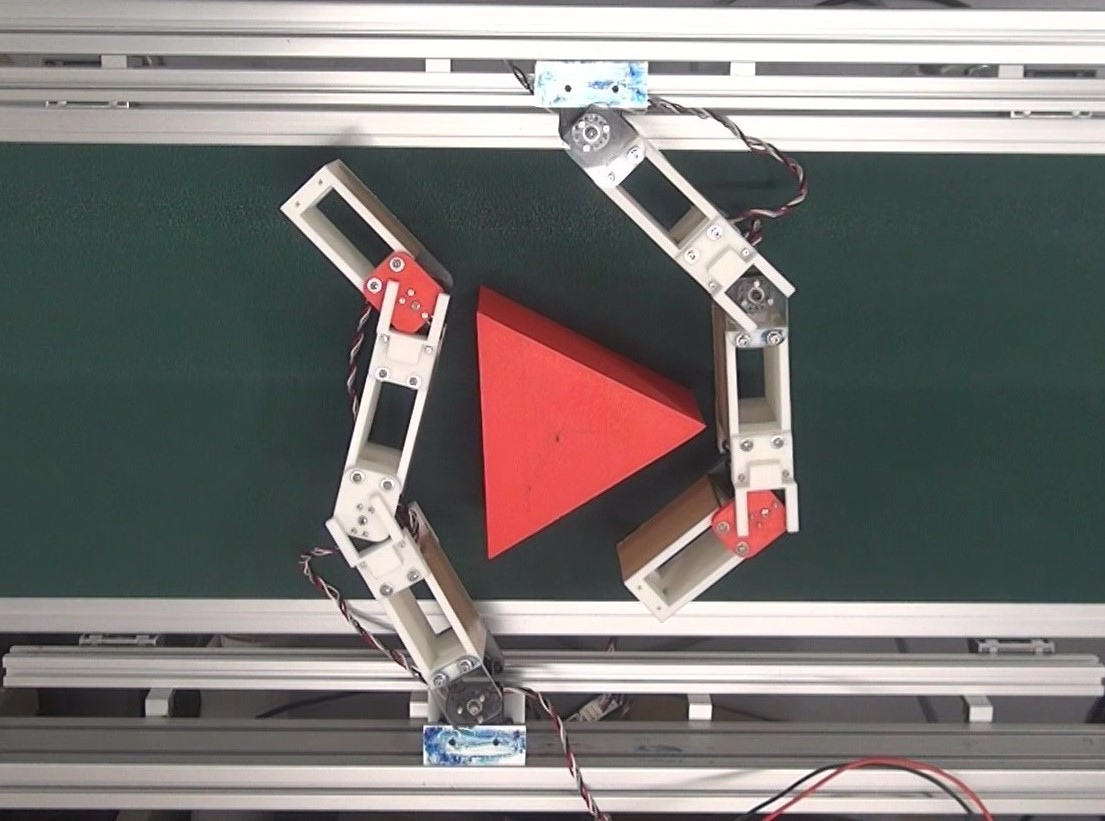
\includegraphics[width=0.9\linewidth]{fig/4-manipulation-result/Triangle/1-1.jpg}
\end{minipage}\hfill
\begin{minipage}{0.249\linewidth}
\centering
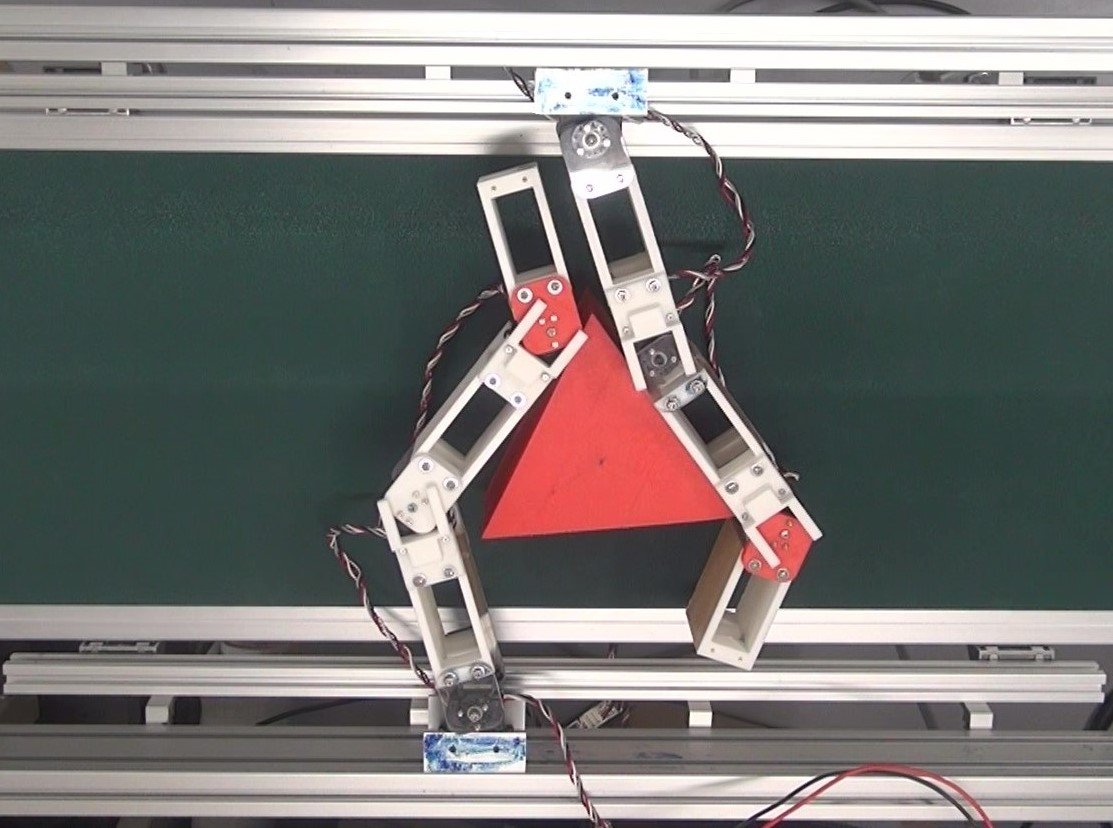
\includegraphics[width=0.9\linewidth]{fig/4-manipulation-result/Triangle/1-2.jpg}
\end{minipage}\hfill
\begin{minipage}{0.249\linewidth}
\centering
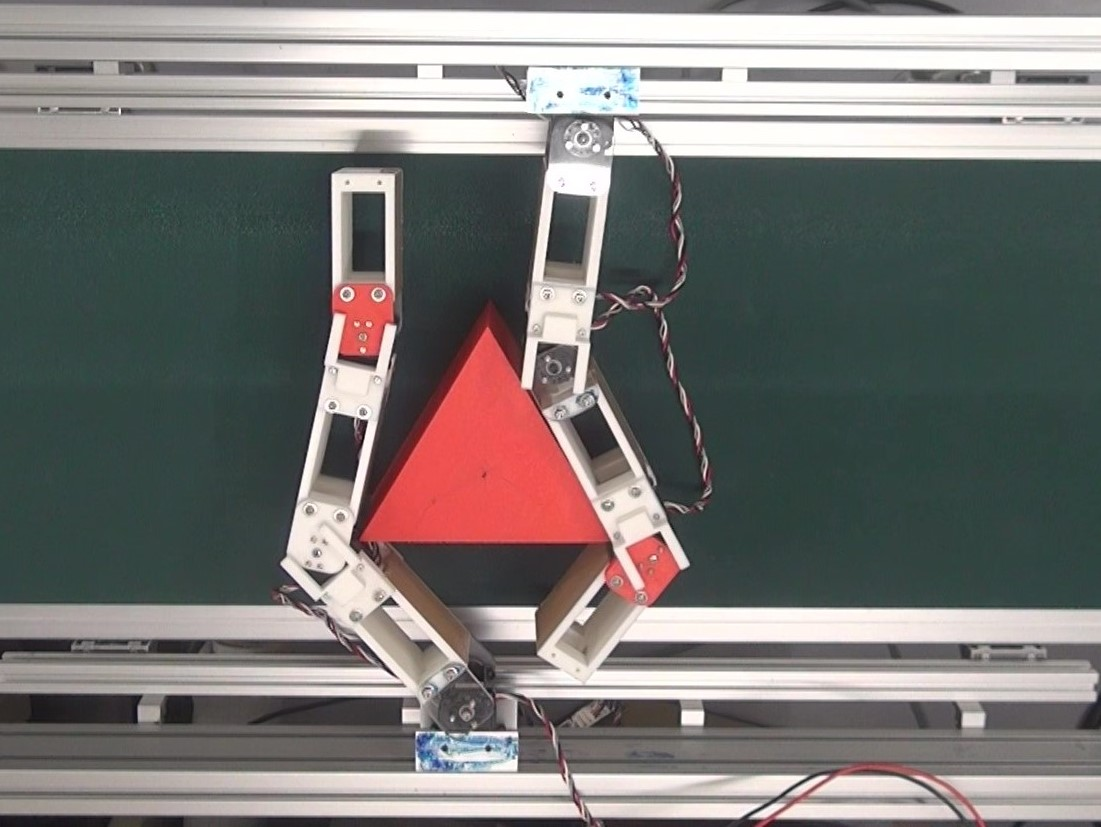
\includegraphics[width=0.9\linewidth]{fig/4-manipulation-result/Triangle/1-3.jpg}
\end{minipage}\hfill
\begin{minipage}{0.249\linewidth}
\centering
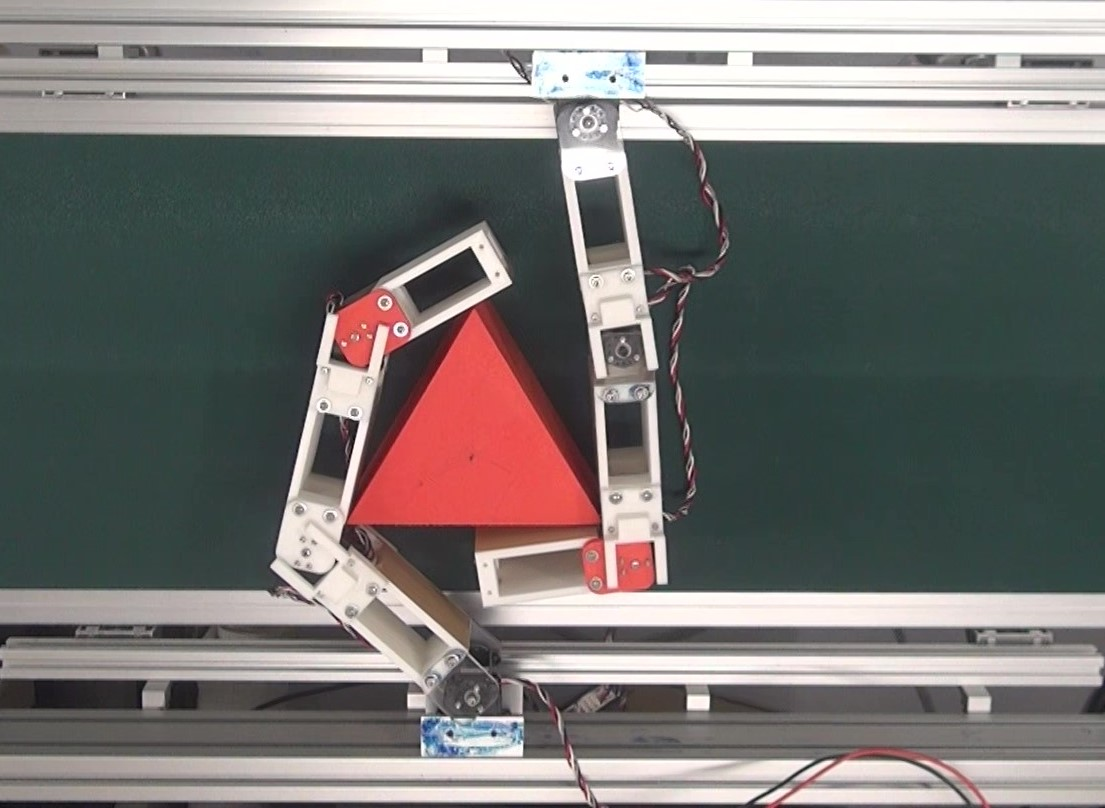
\includegraphics[width=0.9\linewidth]{fig/4-manipulation-result/Triangle/1-4.jpg}
\end{minipage}
\caption{Triangle manipulation result \#1}\label{fig::trim1}

\begin{minipage}{0.249\linewidth}
\centering
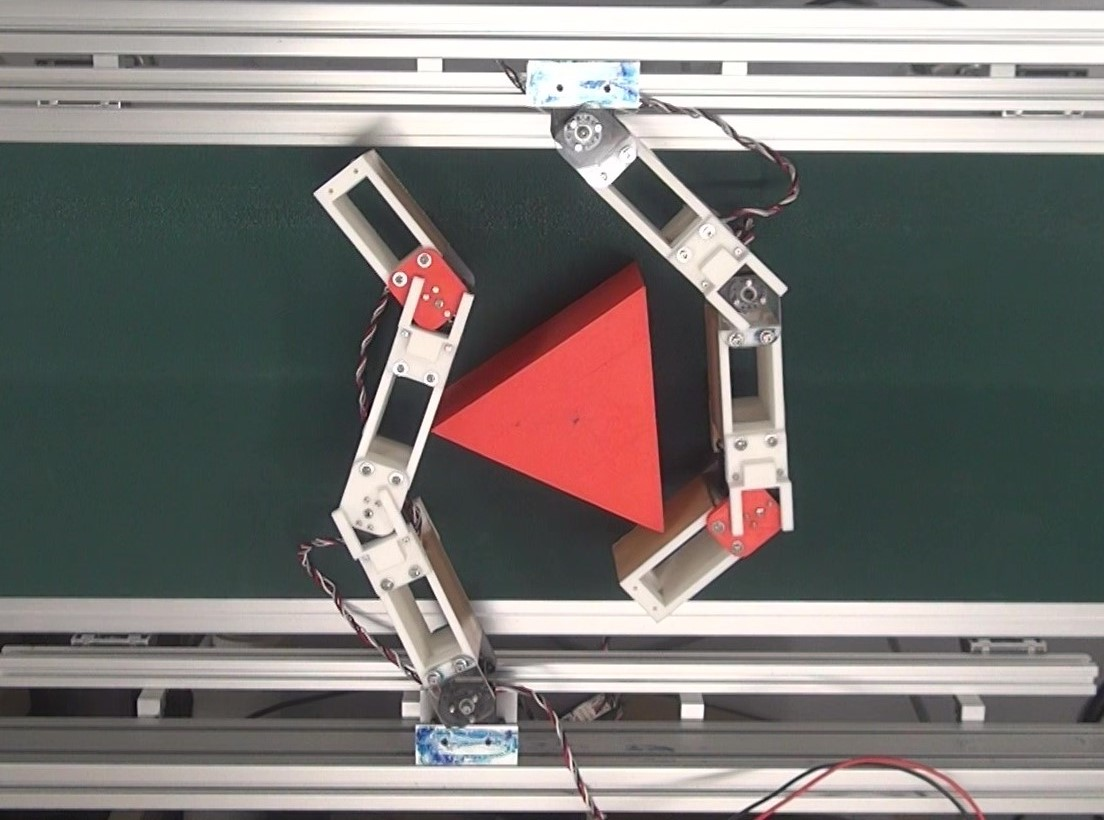
\includegraphics[width=0.9\linewidth]{fig/4-manipulation-result/Triangle/2-1.jpg}
\end{minipage}\hfill
\begin{minipage}{0.249\linewidth}
\centering
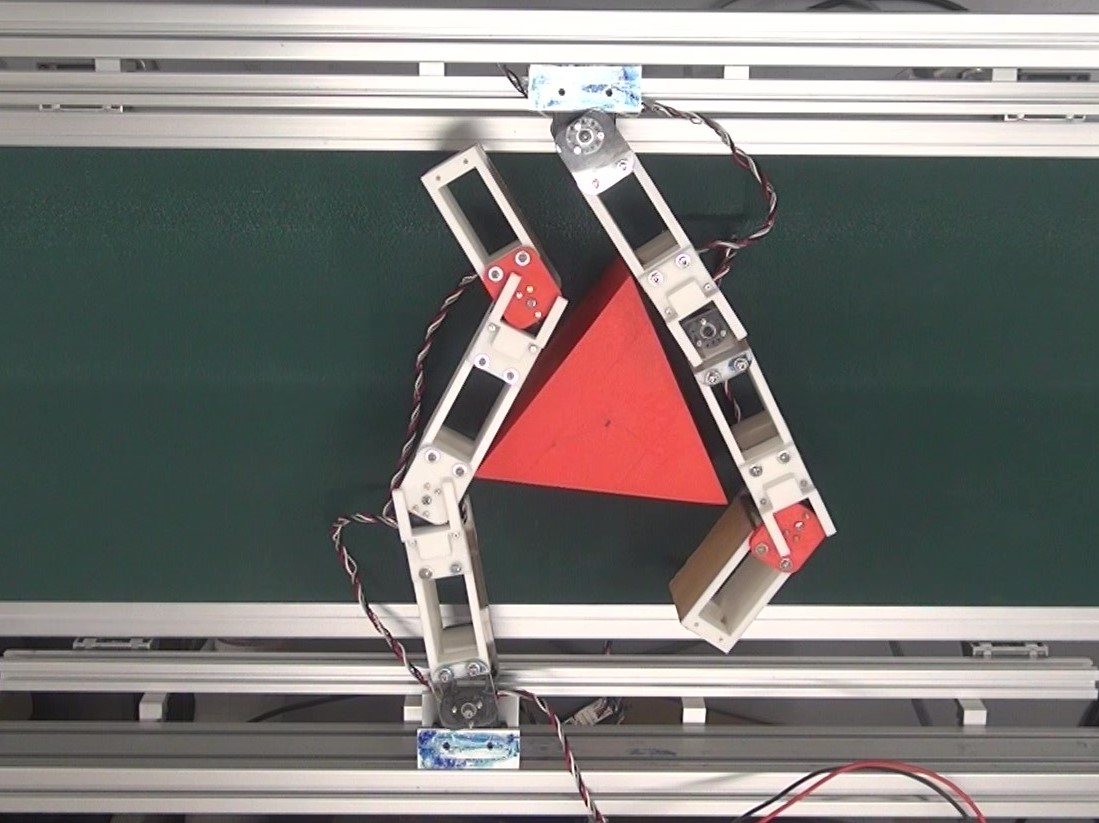
\includegraphics[width=0.9\linewidth]{fig/4-manipulation-result/Triangle/2-2.jpg}
\end{minipage}\hfill
\begin{minipage}{0.249\linewidth}
\centering
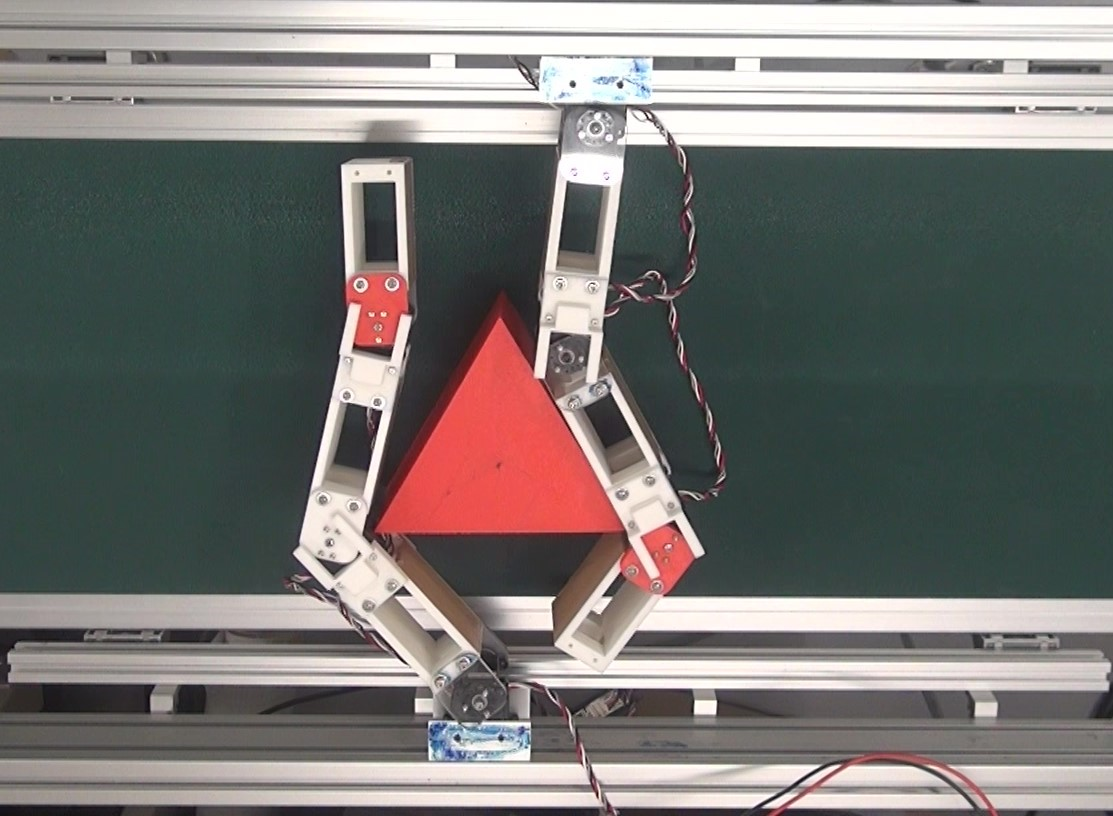
\includegraphics[width=0.9\linewidth]{fig/4-manipulation-result/Triangle/2-3.jpg}
\end{minipage}\hfill
\begin{minipage}{0.249\linewidth}
\centering
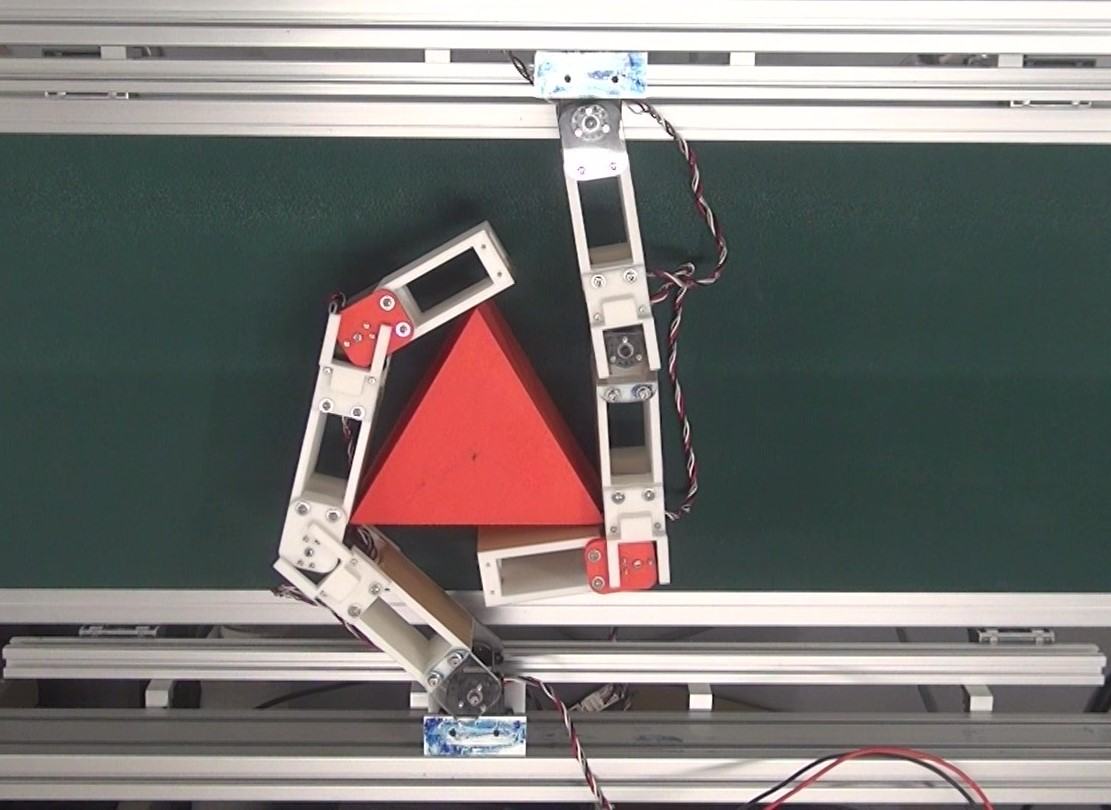
\includegraphics[width=0.9\linewidth]{fig/4-manipulation-result/Triangle/2-4.jpg}
\end{minipage}
\caption{Triangle manipulation result \#2}\label{fig::trim2}

\begin{minipage}{0.249\linewidth}
\centering
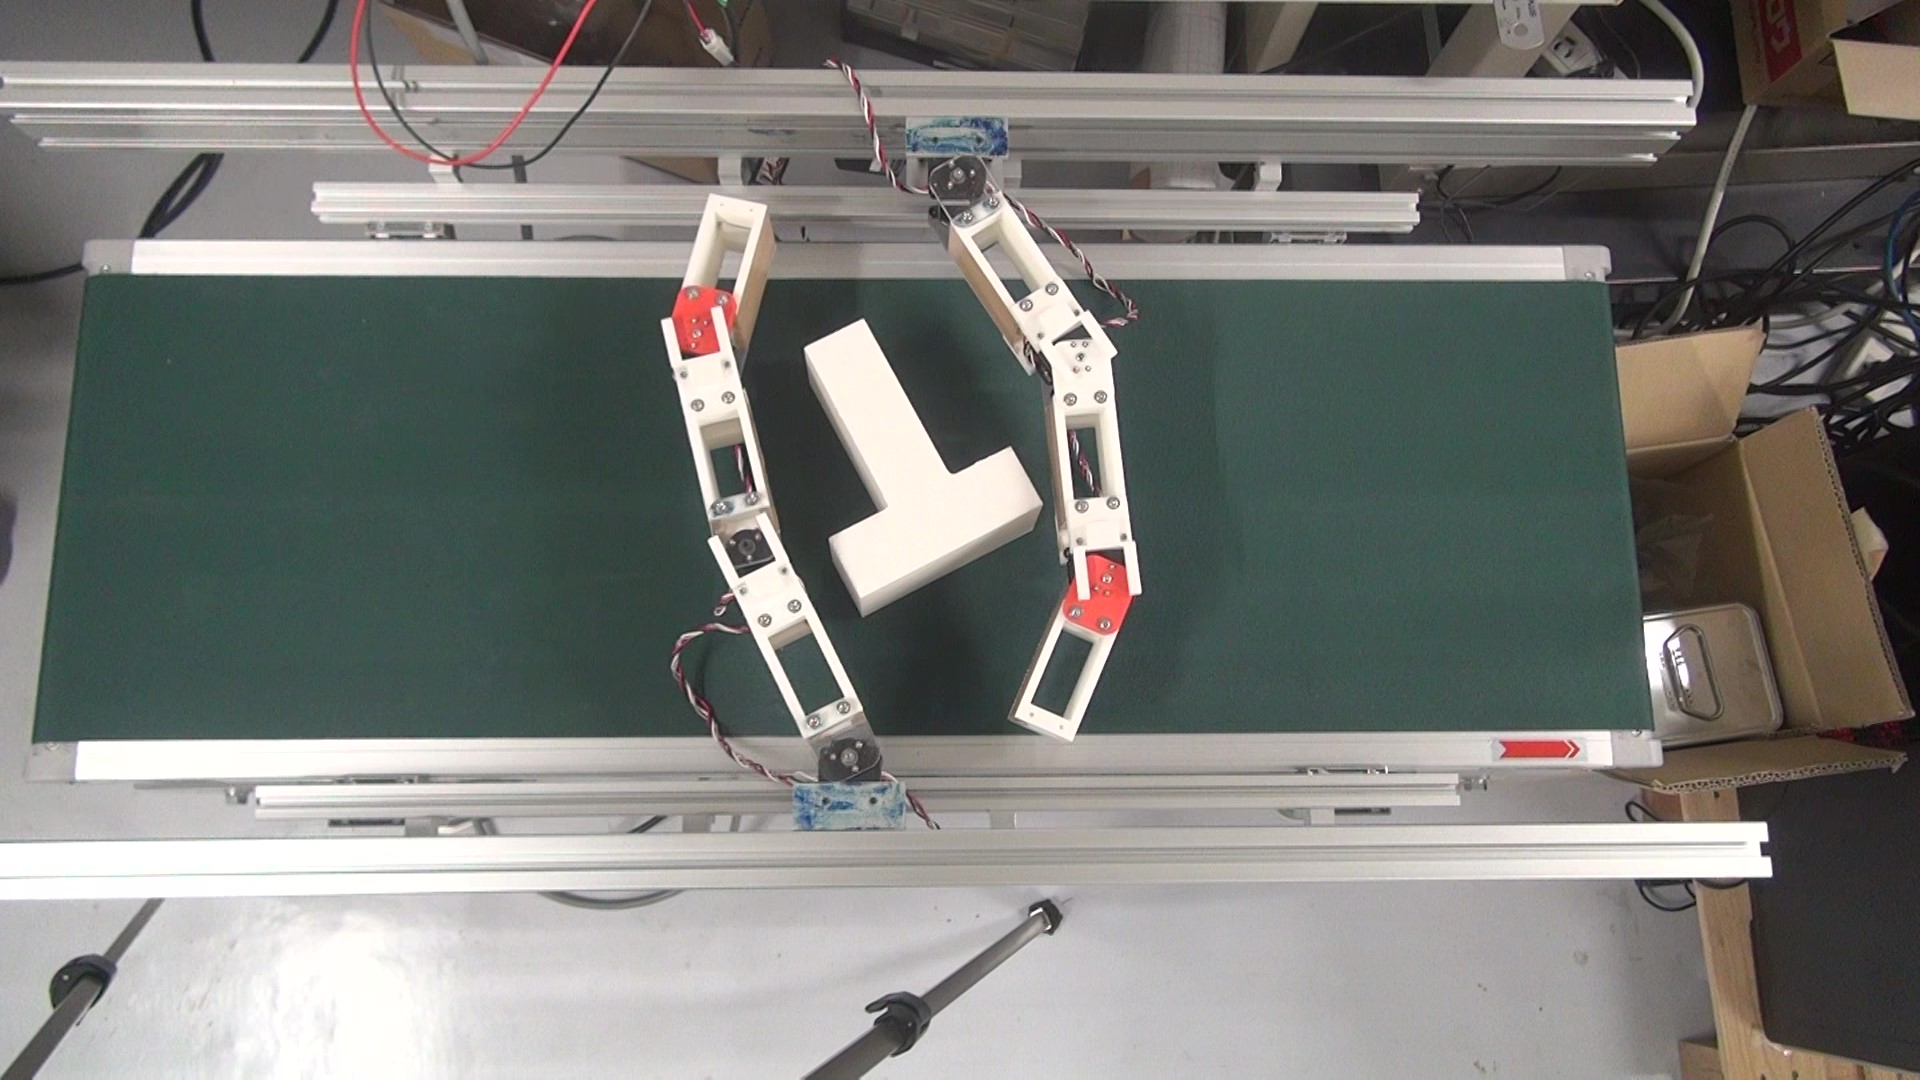
\includegraphics[width=0.9\linewidth]{fig/4-manipulation-result/TShape/1-1.jpg}
\end{minipage}\hfill
\begin{minipage}{0.249\linewidth}
\centering
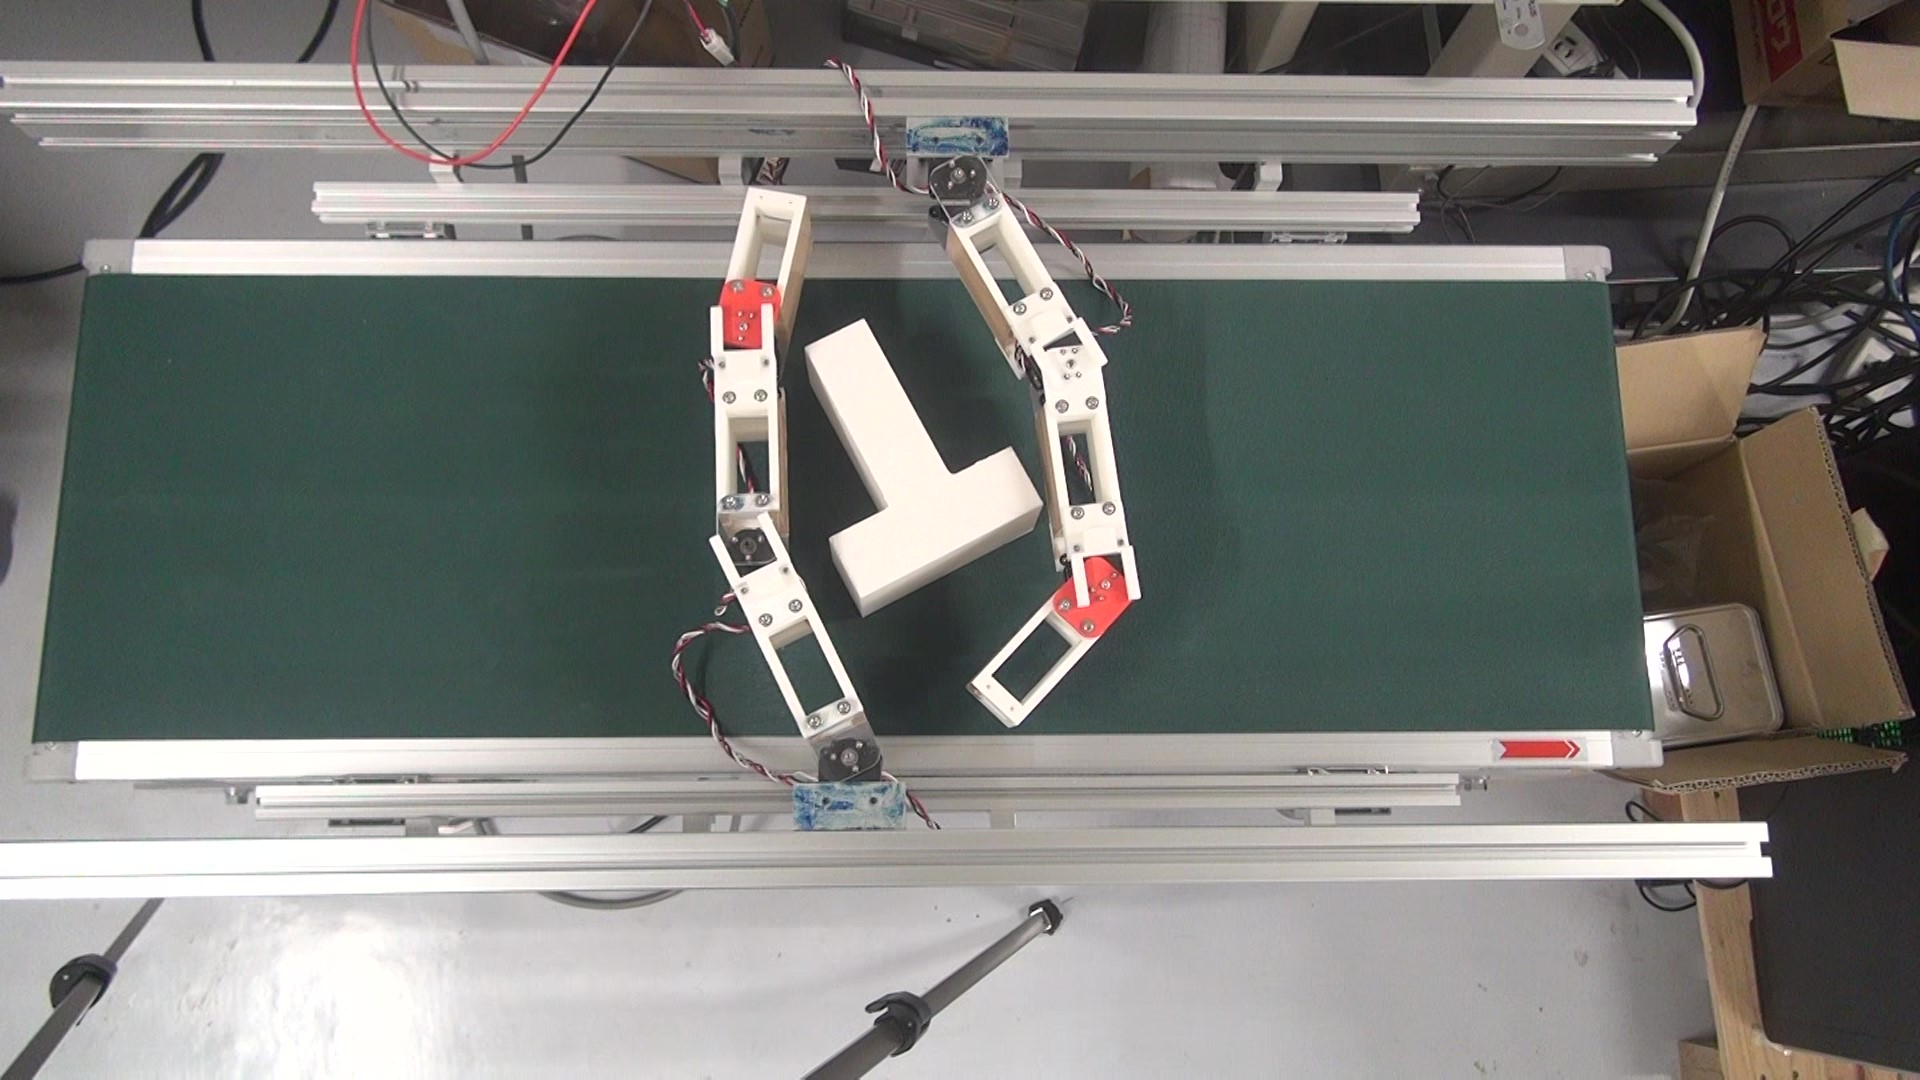
\includegraphics[width=0.9\linewidth]{fig/4-manipulation-result/TShape/1-2.jpg}
\end{minipage}\hfill
\begin{minipage}{0.249\linewidth}
\centering
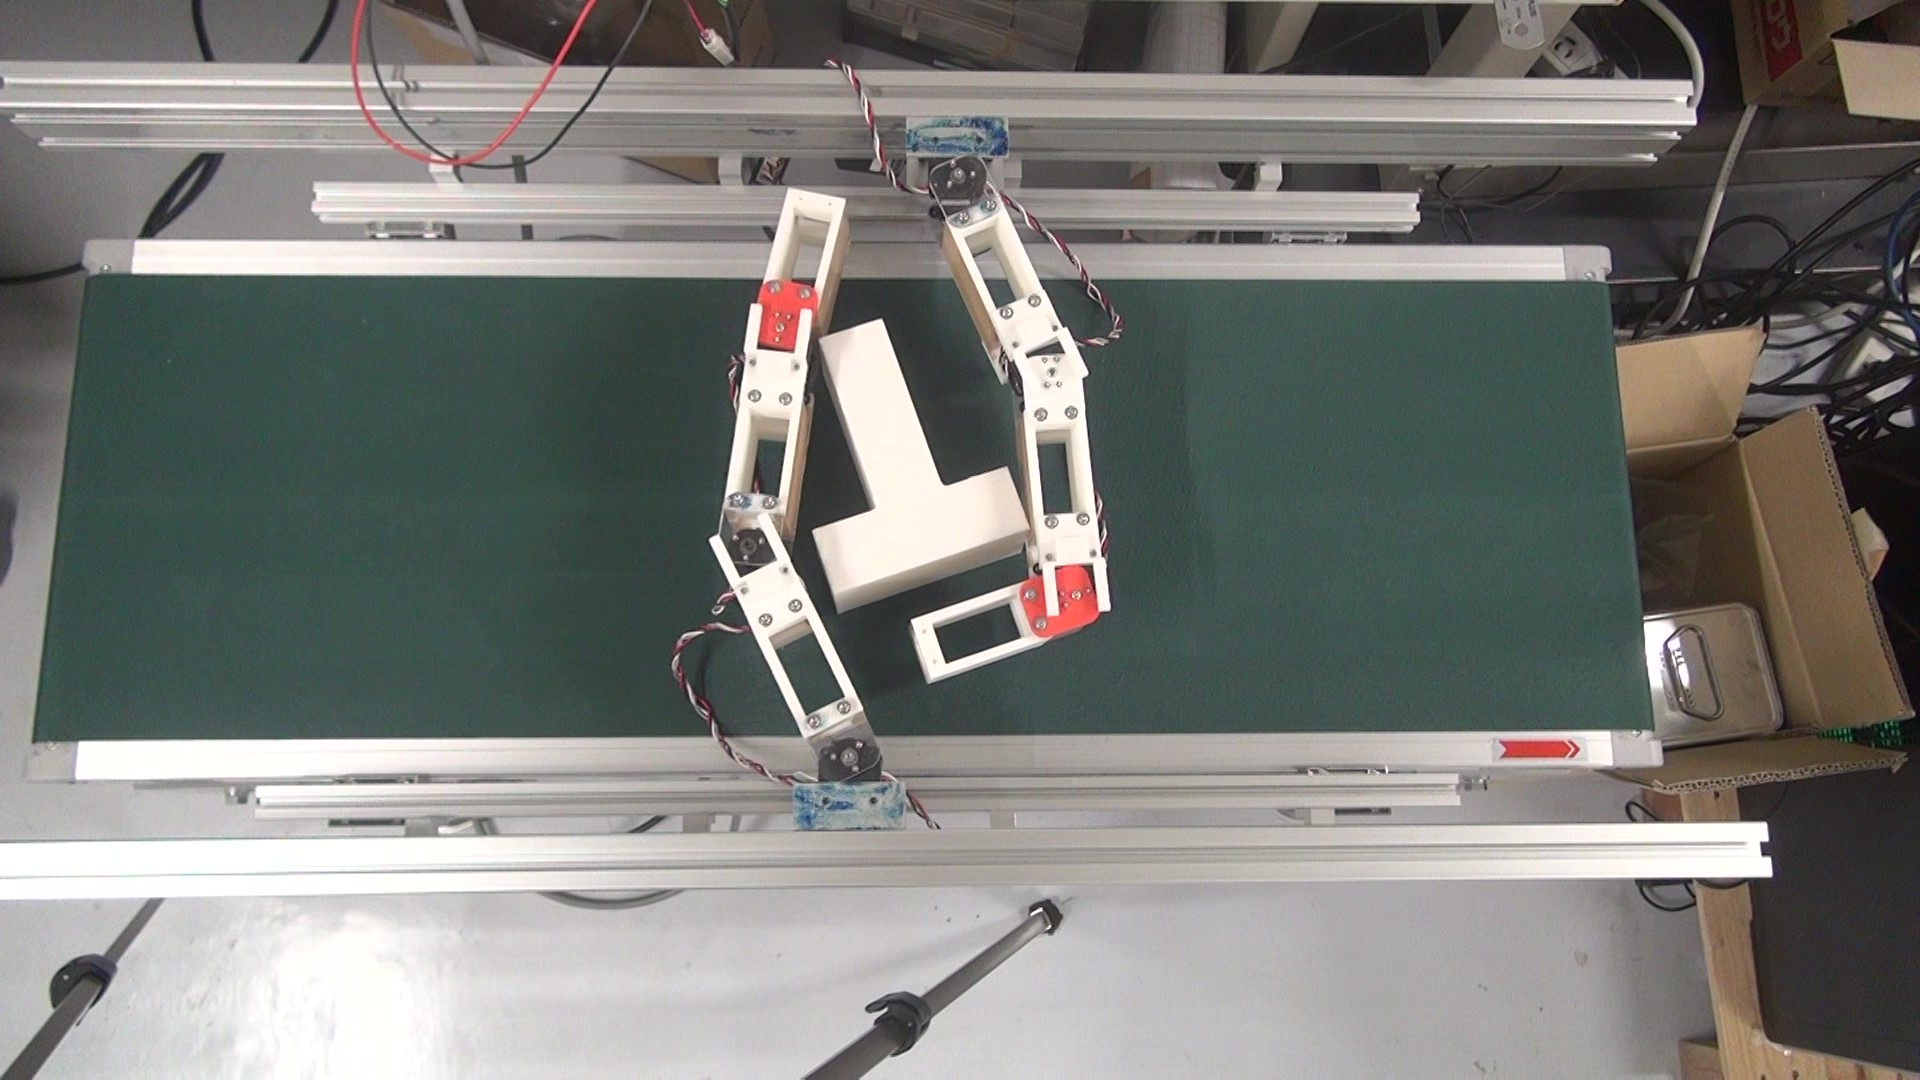
\includegraphics[width=0.9\linewidth]{fig/4-manipulation-result/TShape/1-3.jpg}
\end{minipage}\hfill
\begin{minipage}{0.249\linewidth}
\centering
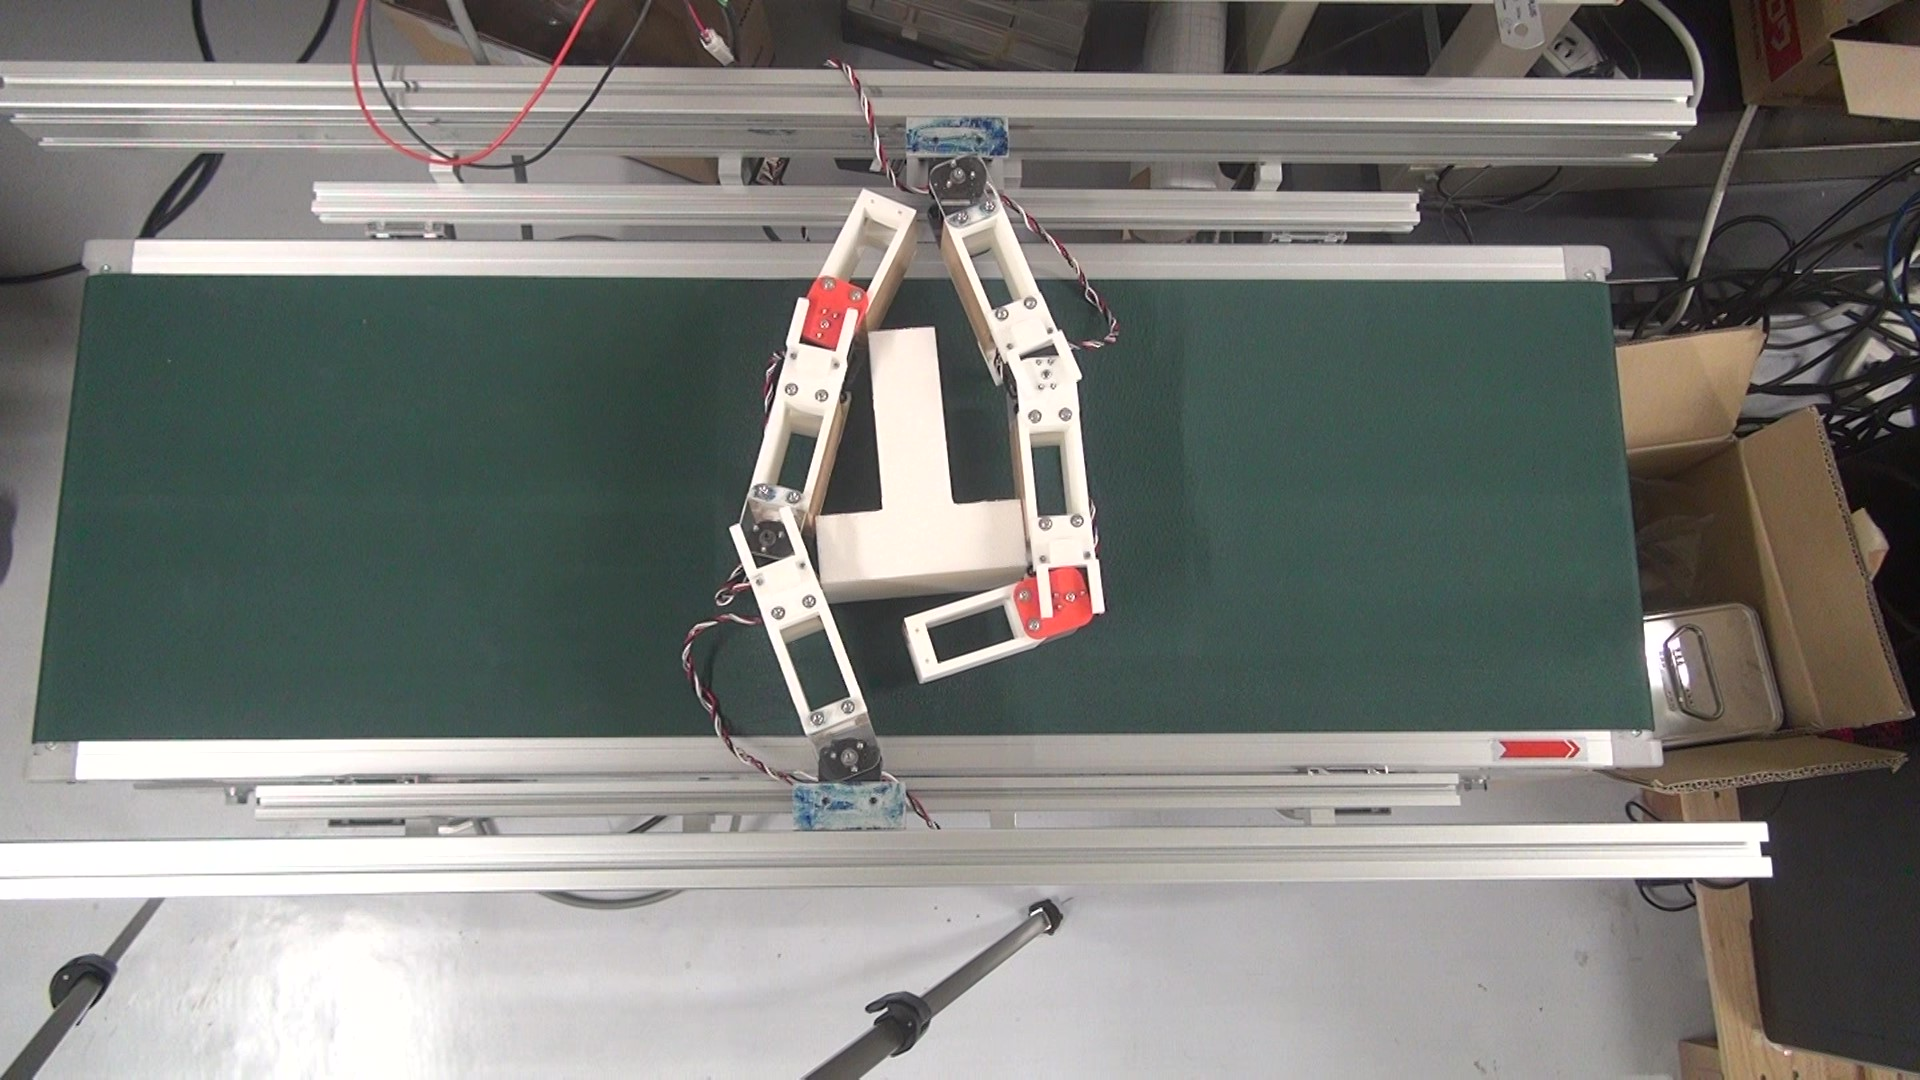
\includegraphics[width=0.9\linewidth]{fig/4-manipulation-result/TShape/1-4.jpg}
\end{minipage}
\caption{T-Shape manipulation result \#1}\label{fig::tm1}

\begin{minipage}{0.249\linewidth}
\centering
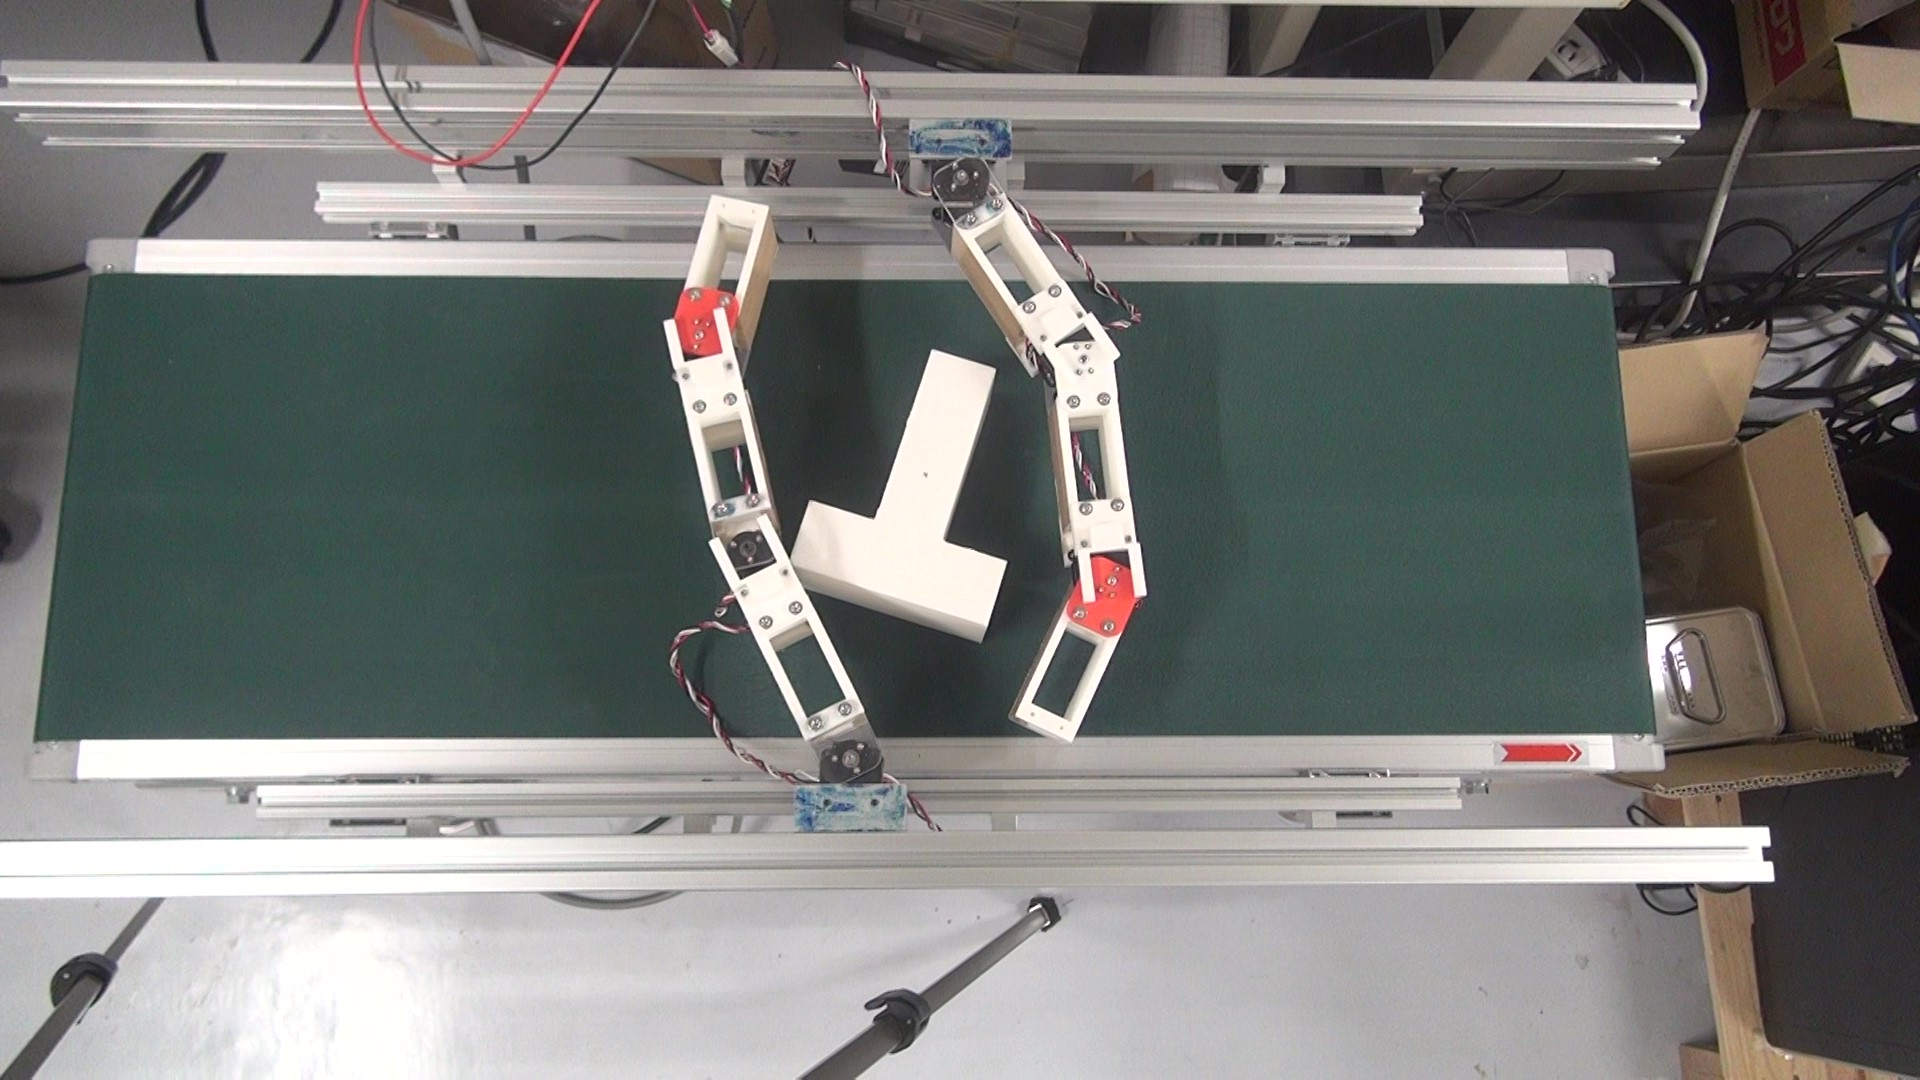
\includegraphics[width=0.9\linewidth]{fig/4-manipulation-result/TShape/2-1.jpg}
\end{minipage}\hfill
\begin{minipage}{0.249\linewidth}
\centering
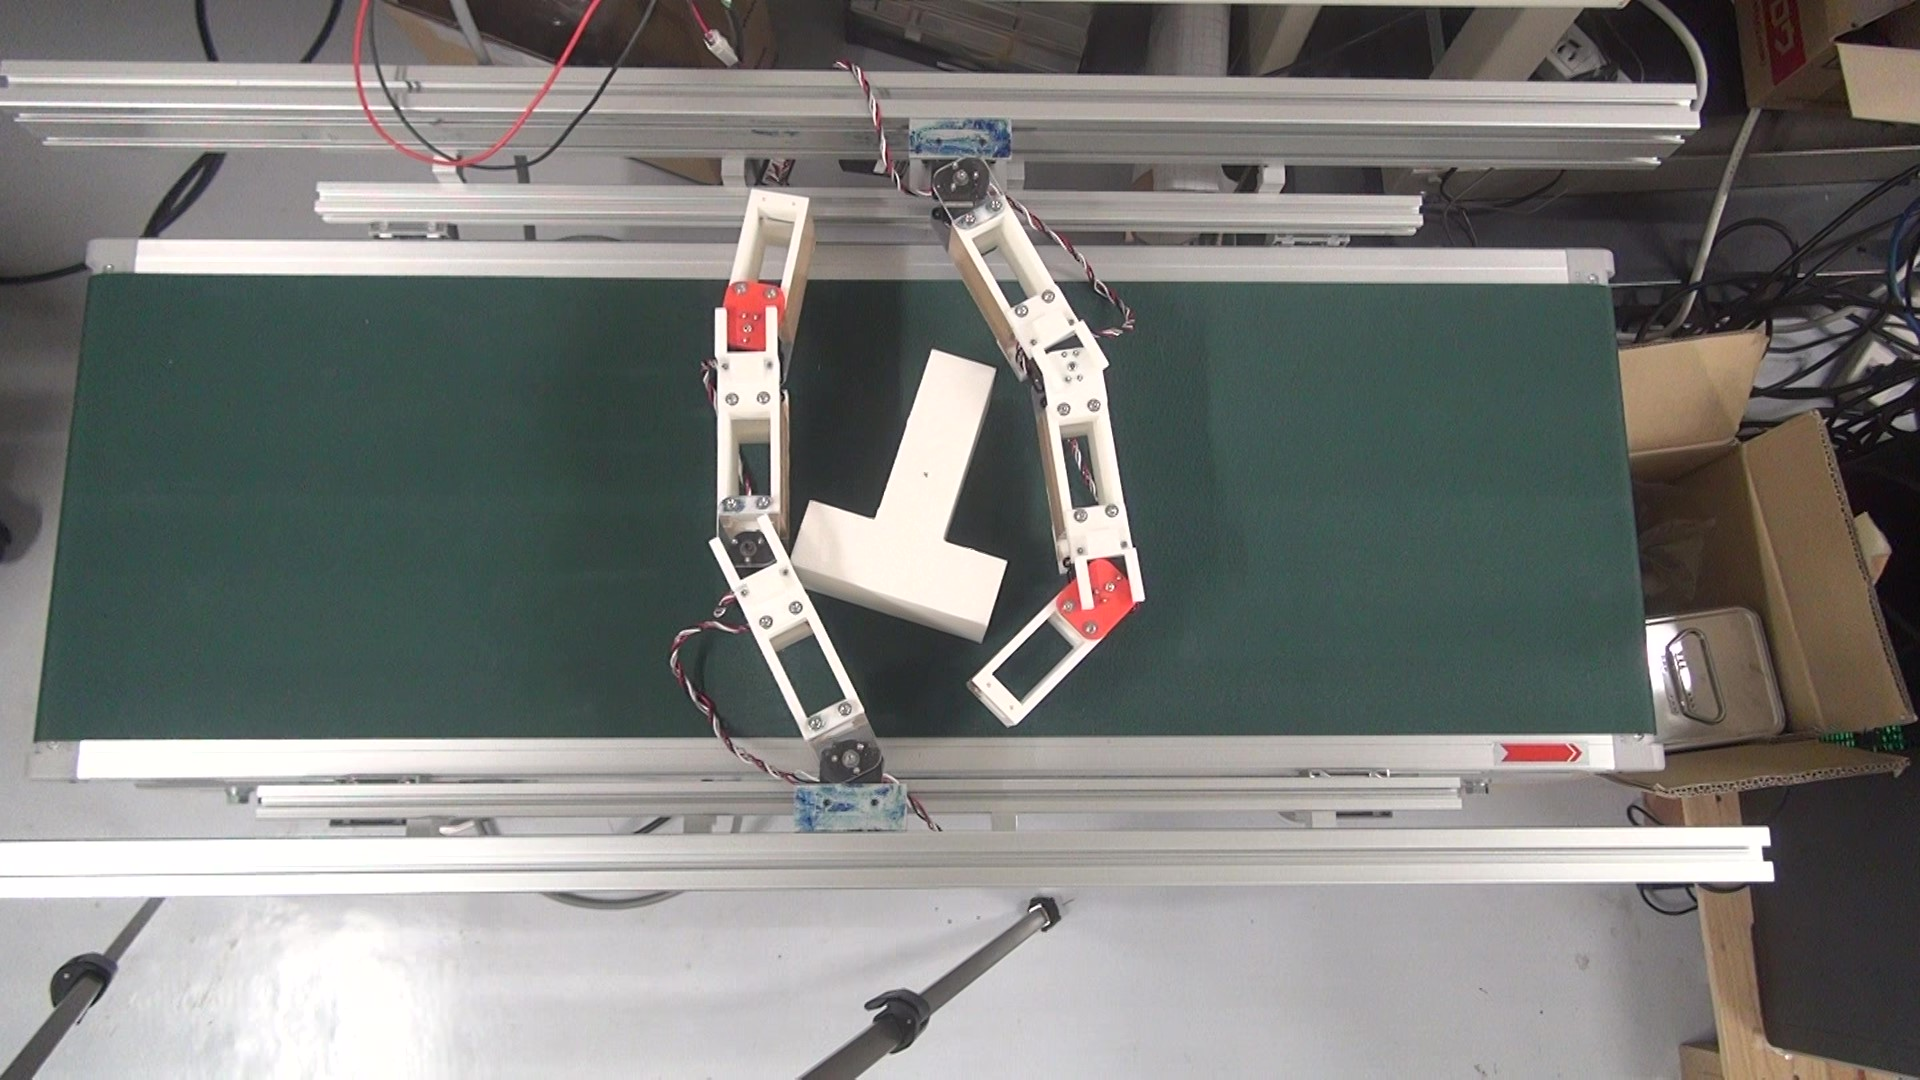
\includegraphics[width=0.9\linewidth]{fig/4-manipulation-result/TShape/2-2.jpg}
\end{minipage}\hfill
\begin{minipage}{0.249\linewidth}
\centering
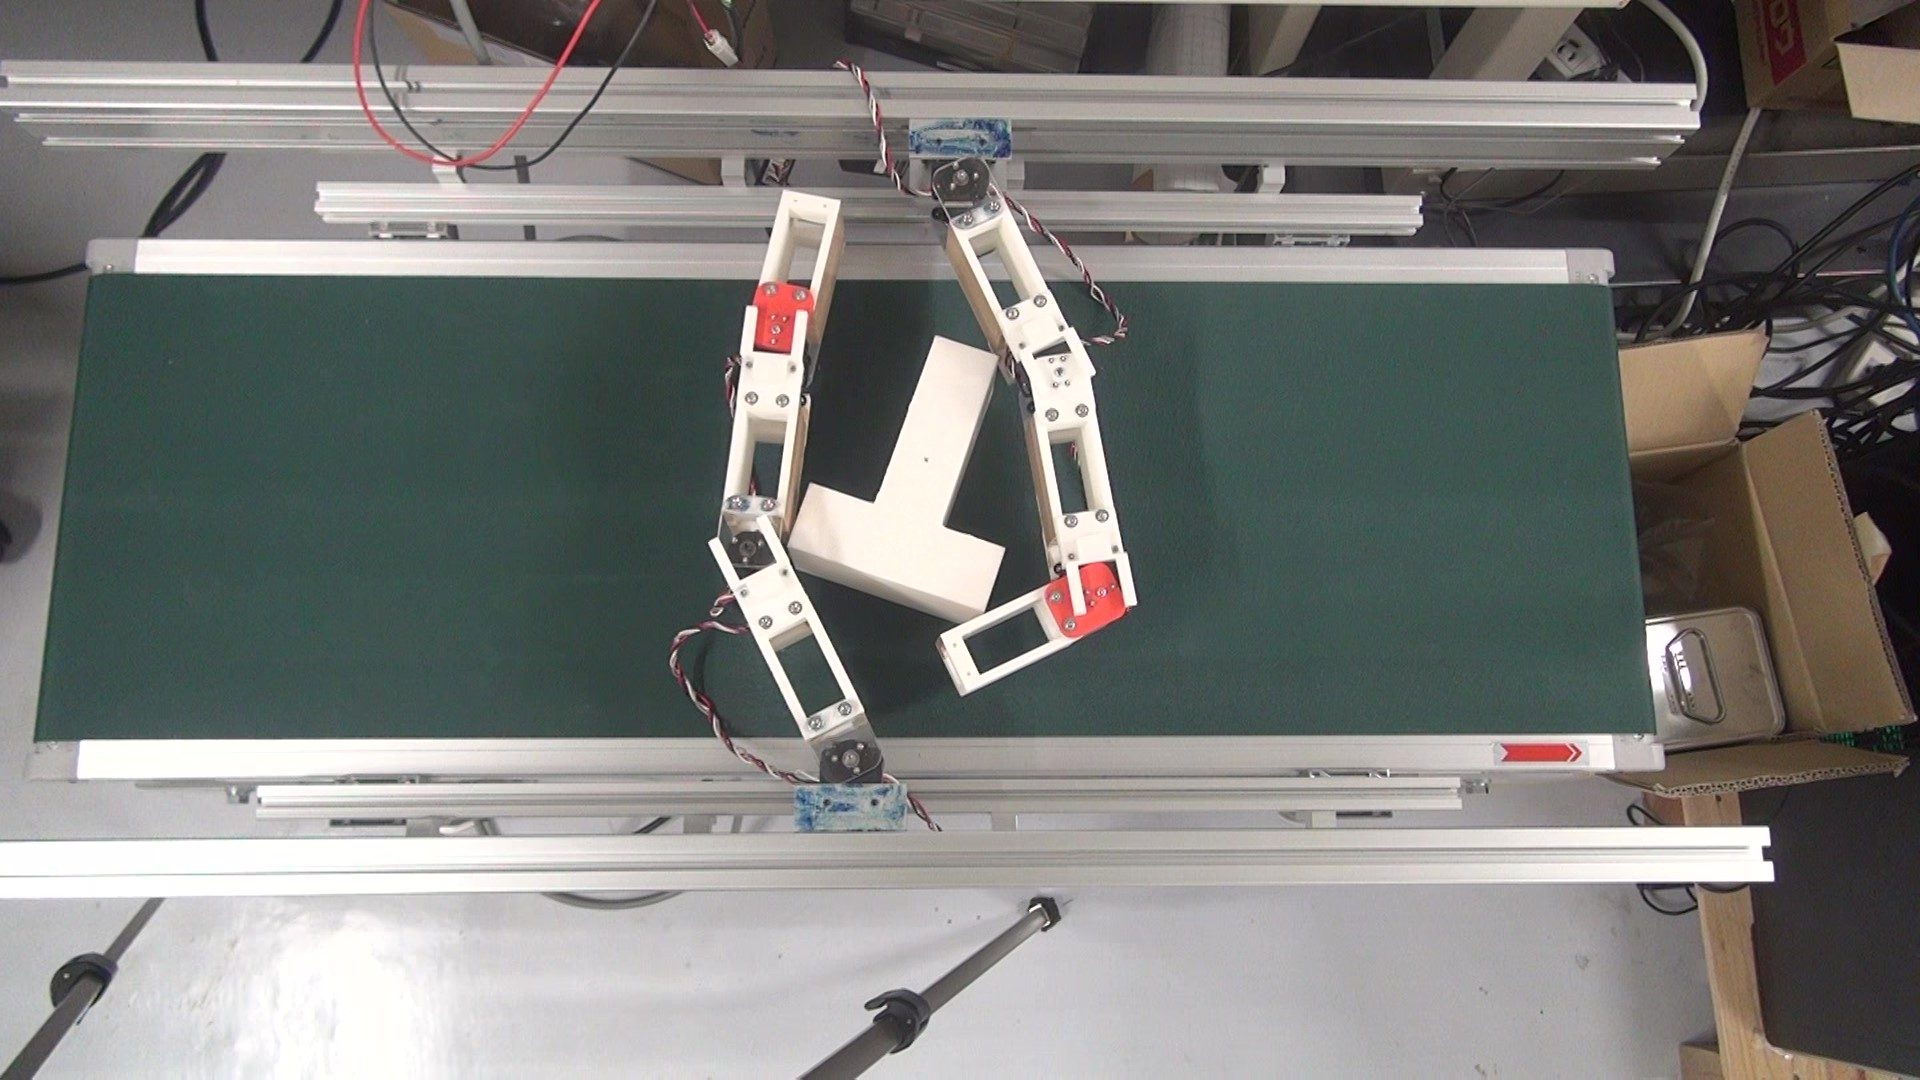
\includegraphics[width=0.9\linewidth]{fig/4-manipulation-result/TShape/2-3.jpg}
\end{minipage}\hfill
\begin{minipage}{0.249\linewidth}
\centering
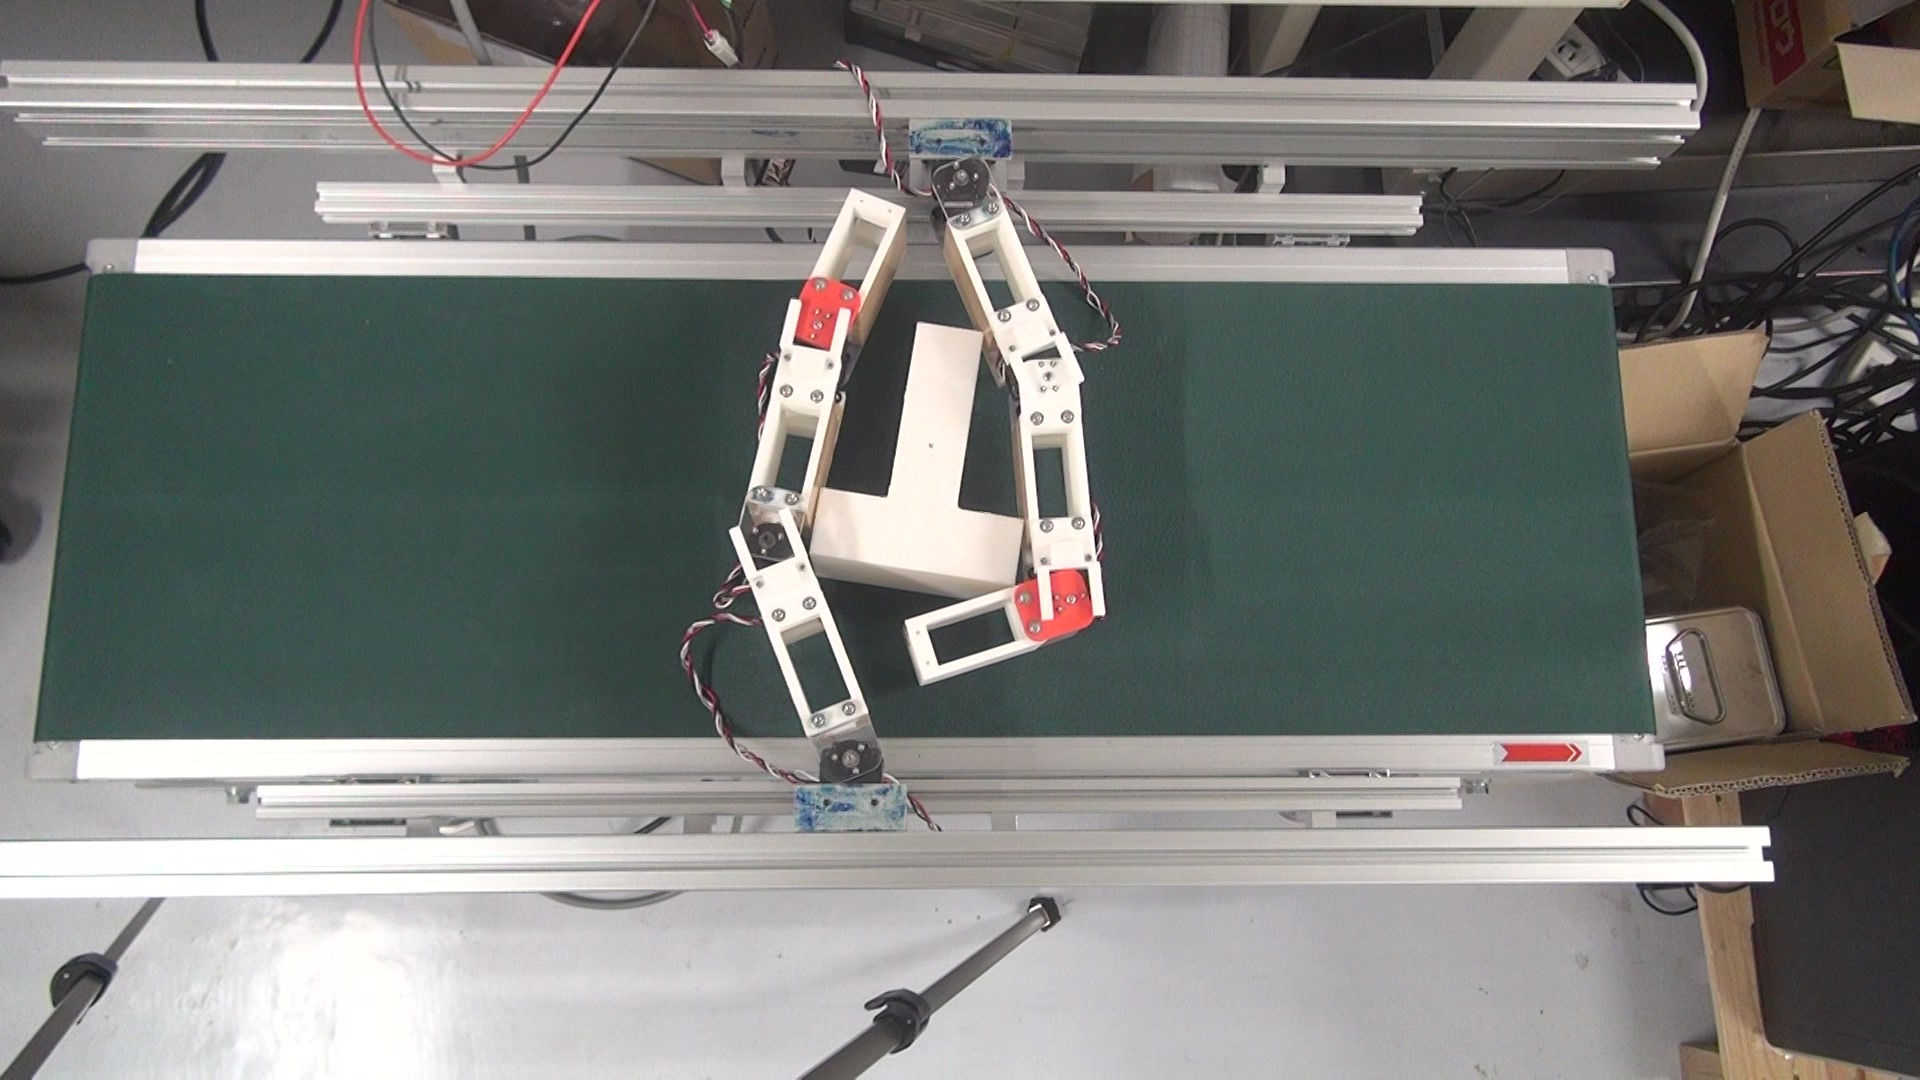
\includegraphics[width=0.9\linewidth]{fig/4-manipulation-result/TShape/2-4.jpg}
\end{minipage}
\caption{T-Shape manipulation result \#2}\label{fig::tm2}
\end{figure}


\section{結論}
汎用パーツフィーダへの応用に向けて,ハード面,ソフト面の両方から,センサレスin-handケージングマニピュレーションの機能向上に取り組んだ.先行研究から問題であったジャミングに関しては,ジャミングの発生原因となっていたパーム部付近のハンド低自由度領域を排した対向型ハンドにより解決した.動作計画では新たに2つのアルゴリズムを提案し,以前から課題であった計算時間の問題を改善した.また,これら3つのアルゴリズムを使い分けることで,ユーザの様々なニーズに対応できるようになった.


%% 参考文献
\begin{thebibliography}{9}
\bibitem[1]{rimon1999} 
E. Rimon, A. Blake:
``Caging Planar Bodies by One-Parameter Two-Fingered Gripping Systems,''
{\it The International Journal of Robotics Research}, Vol.~18, no.~3, pp.~299--318, 1999.

\bibitem[2]{komiyama2021}
込山 隼:
``センサレスin-hand ケージングマニピュレーションによる物体の位置・姿勢制御'',
横浜国立大学大学院理工学府 機械・材料海洋系工学専攻, ポートフォリオ, 2021.

\bibitem[3]{kamikukita2022}
上久木田 治毅:
``センサレス in-hand ケージングマニピュレーションに基づく汎用パーツフィーダの開発'', 
横浜国立大学理工学部 機械・材料・海洋系学科 機械工学EP, 卒業論文, 2022.

%  	\bibitem[]{lavalle2001}
%  	S. M. LaValle, J. J. Kuffner, 
%  	``Rapidly-exploring Random Tree: Progress and Prospects'', 
%  	{\it Algorithmic and Computational Robotics: New Directions 2000 WAFR}, 
%  	in B. R. Donald, K. M. Lynch, and D. Rus, editors, 
%  	pp.~293--308, A K Peters, 2001.
%  	
%  	  	\bibitem[]{kuffner2000}
%%  	Walter G. Bircher, Andrew S. Morgan, Kaiyu Hang, Aaron M. Dollar,
%	J. J. Kuffner, S. M. LaValle, 
%	``RRT-connect: An Efficient Approach to Single-Query Path Planning'',
%	{\it Proceedings 2000 ICRA. Millennium Conference. IEEE International Conference on Robotics and Automation. Symposia Proceedings (Cat. No.00CH37065)}, 
%	 Vol.~2, pp.~995--1001, 2000.

\end{thebibliography}

\end{document}
